\documentclass[a4paper]{article}

\usepackage{showcode/showcode}
\usepackage{multicol}
\usepackage{blindtext}
\usepackage{amssymb}
\usepackage{amsthm}
\usepackage{mathtools}
\usepackage{bm}

\usepackage[a4paper]{geometry}
\usepackage[hidelinks]{hyperref}
\usepackage{eurosym}
\usepackage{caption, subcaption}
\usepackage{tikz, circuitikz}
\usepackage{pgf-umlcd, pgf-umlsd}
\usepackage[italian]{babel} % FIXME
\usepackage[utf8]{inputenc}
\usepackage[T1]{fontenc}
\usepackage[normalem]{ulem}

\renewcommand{\umltextcolor}{black}
\renewcommand{\umldrawcolor}{black}
\renewcommand{\umlfillcolor}{white}

\definecolor{type}{RGB}{132, 42, 17}

\textwidth=450pt
\oddsidemargin=0pt
\textheight=665pt
\voffset=-50pt

\begin{document}

\begin{titlepage}
    \begin{center}
        
\includegraphics[height=5cm]{minerva.pdf}

        \vspace*{1.75cm}

        \LARGE

        \textbf{MSc in Computer Science} \\
        at University of Milan

        \vspace*{1cm}

        \huge
        Emulatore CHIP-8 su STM32

        \large Relazione per il progetto di PROS, \\
        corso tenuto da \textbf{Danilo Bruschi}

        \normalsize
        \vspace*{4cm}

        \begin{minipage}[t]{0.47\textwidth}
            {\large \href{federico.bruzzone@studenti.unimi.it}{federico.bruzzone@studenti.unimi.it}} \vspace{1em}  \\
            {\large \href{lorenzo.ferrante1@studenti.unimi.it}{lorenzo.ferrante1@studenti.unimi.it}} \vspace{1em}  \\
            {\large \href{andrea.longoni3@studenti.unimi.it}{andrea.longoni3@studenti.unimi.it}} \vspace{1em}  \\
        \end{minipage}
        \hfill
        \begin{minipage}[t]{0.47\textwidth}\raggedleft
            {\large \textbf{Federico Bruzzone}} \\
            \vspace{1em}
            {\large \textbf{Lorenzo Ferrante}} \\
            \vspace{1em}
            {\large \textbf{Andrea Longoni}}
        \end{minipage}

        \vfill
        Anno accademico 2022/2023

    \end{center}
\end{titlepage}
\setlength{\parindent}{0pt}
\setlength{\parskip}{0.8em}

\tableofcontents
\listoffigures
\listoftables

\newpage

\begin{center}
\fbox{
    \begin{minipage}{0.9\textwidth}
    \footnotesize\itshape
    Abbiamo deciso di creare un'organizzazione GitHub per rendere accessibile il codice
    sorgente del nostro progetto ad altri programmatori open-source coinvolti con lo sviluppo
    di emulatori e con la community online di CHIP-8.
    \\
    \\
    Link all'organizzazione:
    \begin{itemize}
        \item Macchina virtuale: \url{https://github.com/CHIP-8-Org/Core}
        \item Port su STM32: \url{https://github.com/CHIP-8-Org/STM32-Port}
        \item Documentazione: \url{https://github.com/CHIP-8-Org/Docs}
    \end{itemize}
    \end{minipage}
}
\end{center}

\section{Introduzione}

CHIP-8 è un linguaggio di programmazione creato a metà degli anni '70
da Joseph Weisbecker per semplificare lo sviluppo di videogiochi per
microcomputer a 8 bit. I programmi CHIP-8 vengono interpretati da una
macchina virtuale che è stata estesa parecchie volte nel corso degli
anni, tra le versioni più adottate citiamo S-CHIP e la più recente
XO-CHIP.

La semplicità dell'interprete in aggiunta alla sua lunga storia e
popolarità hanno fatto sì che emulatori e programmi CHIP-8 vengano
realizzati ancora oggi.
Nel corso degli anni molti videogiochi storici sono stati riscritti
in CHIP-8 tra cui Pong, Space Invaders e Tetris.

Lo scopo del progetto è quello di realizzare un emulatore CHIP-8 e
S-CHIP in grado di funzionare su un microcontrollore STM32.

In questo documento ci riferiremo alla macchina virtuale che
interpreta programmi CHIP-8 con "interprete". Mentre utilizzeremo
"emulatore" per indicare l'interprete assieme ad una sua
implementazione (o "port"), ovvero un programma che gestisce
l'audio, il video, l'input da tastiera e interagisce con l'API della
macchina virtuale.

\section{Stato dell'arte}

Al giorno d'oggi risulta difficile ottenere un numero esatto di utenti che
utilizzano CHIP-8,un buon indicatore può essere il topic "chip8" di GitHub
che raggruppa quasi un migliaio di repository.

Tra queste la più popolare è Octo, un'implementazione scritta in JavaScript
capace di eseguire la versione base di CHIP-8, S-CHIP e XO-CHIP nel browser.
La repository è mantenuta da John Earnest, l'inventore di XO-CHIP che nel 2014
ha riportato in vita CHIP-8 modernizzandolo e aggiungendo nuove funzionalità.

Inoltre ogni anno viene organizzata la Octojam, una game jam dove ogni partecipante
prova a sviluppare un videogioco per CHIP-8 (o per le sue estensioni) partendo da zero.

Grazie al suo instruction set ridotto e alla sua limitata richiesta di risorse hardware
è stato portato su un elevato numero di piattaforme, tra cui il Game Boy Color, calcolatrici
grafiche serie HP 48 e Emacs (il famoso editor di testo).

Sebbene CHIP-8 e S-CHIP siano stati tradizionalmente implementati tramite software
esistono anche implementazioni hardware. Ne citiamo una in particolare scritta nel
linguaggio Verilog per schede FPGA.

\section{Hardware}\label{sec:hardware}

\begin{figure}[h!t]
    \begin{subfigure}[b]{0.45\textwidth}
        \begin{center}
            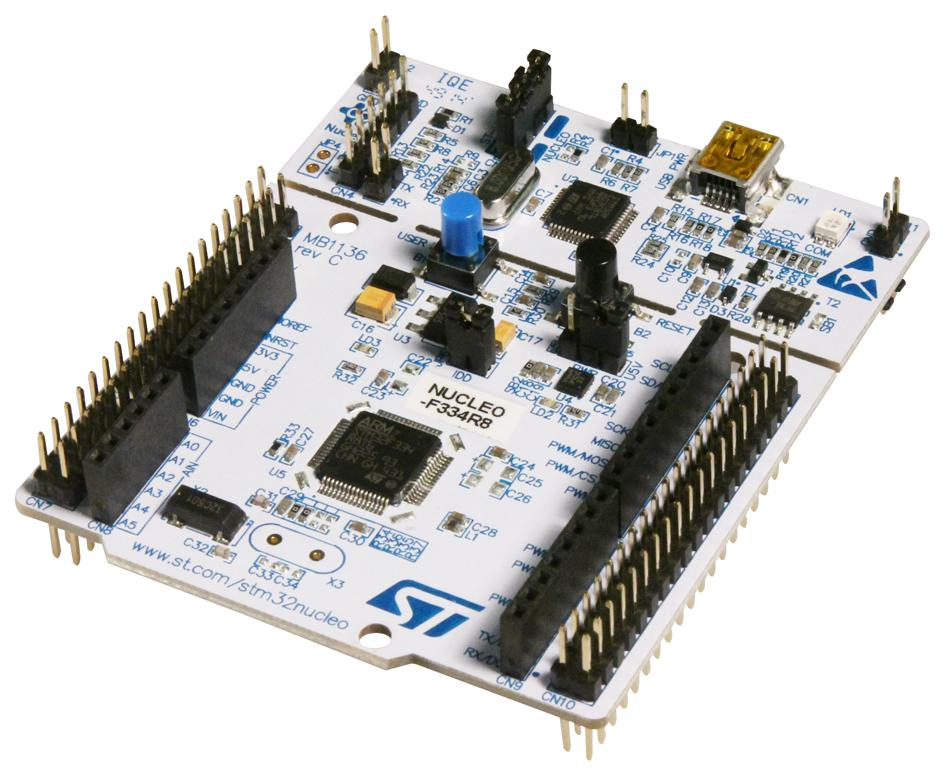
\includegraphics[scale=0.15]{figures/stm32f334.jpg}
        \end{center}
        \caption{Il microcontrollore \texttt{STM32F334R8T6}.}
        \label{fig:stm32f334}
    \end{subfigure}
    \hfill
    \begin{subfigure}[b]{0.45\textwidth}
        \begin{center}
            \begin{tikzpicture}[x=0.015cm, y=0.015cm, scale=0.50, transform shape]
                % \draw  [color={rgb, 255:red, 0; green, 0; blue, 0 }  ,draw opacity=1 ][fill={rgb, 255:red, 255; green, 255; blue, 255 }  ,fill opacity=1 ] (400,140) -- (720,140) -- (720,960) -- (400,960) -- cycle ;
\draw  [color={rgb, 255:red, 0; green, 0; blue, 0 }  ,draw opacity=1 ][fill={rgb, 255:red, 255; green, 255; blue, 255 }  ,fill opacity=1 ] (400,140) -- (720,140) -- (720,920) -- (400,920) -- cycle ;

\draw  [fill={rgb, 255:red, 255; green, 255; blue, 255 }  ,fill opacity=1 ] (440,150) -- (510,150) -- (510,190) -- (440,190) -- cycle ;
\draw  [fill={rgb, 255:red, 255; green, 255; blue, 255 }  ,fill opacity=1 ] (370,150) -- (440,150) -- (440,190) -- (370,190) -- cycle ;

\draw  [fill={rgb, 255:red, 255; green, 255; blue, 255 }  ,fill opacity=1 ] (440,190) -- (510,190) -- (510,230) -- (440,230) -- cycle ;
\draw  [fill={rgb, 255:red, 255; green, 255; blue, 255 }  ,fill opacity=1 ] (370,190) -- (440,190) -- (440,230) -- (370,230) -- cycle ;

\draw  [fill={rgb, 255:red, 255; green, 255; blue, 255 }  ,fill opacity=1 ] (440,230) -- (510,230) -- (510,270) -- (440,270) -- cycle ;
\draw  [fill={rgb, 255:red, 255; green, 255; blue, 255 }  ,fill opacity=1 ] (370,230) -- (440,230) -- (440,270) -- (370,270) -- cycle ;

\draw  [fill={rgb, 255:red, 255; green, 255; blue, 255 }  ,fill opacity=1 ] (440,270) -- (510,270) -- (510,310) -- (440,310) -- cycle ;
\draw  [fill={rgb, 255:red, 255; green, 255; blue, 255 }  ,fill opacity=1 ] (370,270) -- (440,270) -- (440,310) -- (370,310) -- cycle ;

\draw  [fill={rgb, 255:red, 255; green, 255; blue, 255 }  ,fill opacity=1 ] (440,310) -- (510,310) -- (510,350) -- (440,350) -- cycle ;
\draw  [fill={rgb, 255:red, 255; green, 255; blue, 255 }  ,fill opacity=1 ] (370,310) -- (440,310) -- (440,350) -- (370,350) -- cycle ;

\draw  [fill={rgb, 255:red, 255; green, 255; blue, 255 }  ,fill opacity=1 ] (440,350) -- (510,350) -- (510,390) -- (440,390) -- cycle ;
\draw  [fill={rgb, 255:red, 255; green, 255; blue, 255 }  ,fill opacity=1 ] (370,350) -- (440,350) -- (440,390) -- (370,390) -- cycle ;

\draw  [fill={rgb, 255:red, 255; green, 255; blue, 255 }  ,fill opacity=1 ] (440,390) -- (510,390) -- (510,430) -- (440,430) -- cycle ;
\draw  [fill={rgb, 255:red, 255; green, 255; blue, 255 }  ,fill opacity=1 ] (370,390) -- (440,390) -- (440,430) -- (370,430) -- cycle ;

\draw  [fill={rgb, 255:red, 255; green, 255; blue, 255 }  ,fill opacity=1 ] (440,430) -- (510,430) -- (510,470) -- (440,470) -- cycle ;
\draw  [fill={rgb, 255:red, 255; green, 255; blue, 255 }  ,fill opacity=1 ] (370,430) -- (440,430) -- (440,470) -- (370,470) -- cycle ;

\draw  [fill={rgb, 255:red, 255; green, 255; blue, 255 }  ,fill opacity=1 ] (440,470) -- (510,470) -- (510,510) -- (440,510) -- cycle ;
\draw  [fill={rgb, 255:red, 255; green, 255; blue, 255 }  ,fill opacity=1 ] (370,470) -- (440,470) -- (440,510) -- (370,510) -- cycle ;

\draw  [fill={rgb, 255:red, 255; green, 255; blue, 255 }  ,fill opacity=1 ] (440,510) -- (510,510) -- (510,550) -- (440,550) -- cycle ;
\draw  [fill={rgb, 255:red, 255; green, 255; blue, 255 }  ,fill opacity=1 ] (370,510) -- (440,510) -- (440,550) -- (370,550) -- cycle ;

\draw  [fill={rgb, 255:red, 255; green, 255; blue, 255 }  ,fill opacity=1 ] (440,550) -- (510,550) -- (510,590) -- (440,590) -- cycle ;
\draw  [fill={rgb, 255:red, 255; green, 255; blue, 255 }  ,fill opacity=1 ] (370,550) -- (440,550) -- (440,590) -- (370,590) -- cycle ;

\draw  [fill={rgb, 255:red, 255; green, 255; blue, 255 }  ,fill opacity=1 ] (440,590) -- (510,590) -- (510,630) -- (440,630) -- cycle ;
\draw  [fill={rgb, 255:red, 255; green, 255; blue, 255 }  ,fill opacity=1 ] (370,590) -- (440,590) -- (440,630) -- (370,630) -- cycle ;

\draw  [fill={rgb, 255:red, 255; green, 255; blue, 255 }  ,fill opacity=1 ] (440,630) -- (510,630) -- (510,670) -- (440,670) -- cycle ;
\draw  [fill={rgb, 255:red, 255; green, 255; blue, 255 }  ,fill opacity=1 ] (370,630) -- (440,630) -- (440,670) -- (370,670) -- cycle ;

\draw  [fill={rgb, 255:red, 255; green, 255; blue, 255 }  ,fill opacity=1 ] (440,670) -- (510,670) -- (510,710) -- (440,710) -- cycle ;
\draw  [fill={rgb, 255:red, 255; green, 255; blue, 255 }  ,fill opacity=1 ] (370,670) -- (440,670) -- (440,710) -- (370,710) -- cycle ;

\draw  [fill={rgb, 255:red, 255; green, 255; blue, 255 }  ,fill opacity=1 ] (440,710) -- (510,710) -- (510,750) -- (440,750) -- cycle ;
\draw  [fill={rgb, 255:red, 255; green, 255; blue, 255 }  ,fill opacity=1 ] (370,710) -- (440,710) -- (440,750) -- (370,750) -- cycle ;

\draw  [fill={rgb, 255:red, 255; green, 255; blue, 255 }  ,fill opacity=1 ] (440,750) -- (510,750) -- (510,790) -- (440,790) -- cycle ;
\draw  [fill={rgb, 255:red, 255; green, 255; blue, 255 }  ,fill opacity=1 ] (370,750) -- (440,750) -- (440,790) -- (370,790) -- cycle ;

\draw  [fill={rgb, 255:red, 255; green, 255; blue, 255 }  ,fill opacity=1 ] (440,790) -- (510,790) -- (510,830) -- (440,830) -- cycle ;
\draw  [fill={rgb, 255:red, 255; green, 255; blue, 255 }  ,fill opacity=1 ] (370,790) -- (440,790) -- (440,830) -- (370,830) -- cycle ;

\draw  [fill={rgb, 255:red, 255; green, 255; blue, 255 }  ,fill opacity=1 ] (440,830) -- (510,830) -- (510,870) -- (440,870) -- cycle ;
\draw  [fill={rgb, 255:red, 255; green, 255; blue, 255 }  ,fill opacity=1 ] (370,830) -- (440,830) -- (440,870) -- (370,870) -- cycle ;

\draw  [fill={rgb, 255:red, 255; green, 255; blue, 255 }  ,fill opacity=1 ] (440,870) -- (510,870) -- (510,910) -- (440,910) -- cycle ;
\draw  [fill={rgb, 255:red, 255; green, 255; blue, 255 }  ,fill opacity=1 ] (370,870) -- (440,870) -- (440,910) -- (370,910) -- cycle ;

% \draw  [fill={rgb, 255:red, 255; green, 255; blue, 255 }  ,fill opacity=1 ] (440,910) -- (510,910) -- (510,950) -- (440,950) -- cycle ;
% \draw  [fill={rgb, 255:red, 255; green, 255; blue, 255 }  ,fill opacity=1 ] (370,910) -- (440,910) -- (440,950) -- (370,950) -- cycle ;



\draw  [fill={rgb, 255:red, 255; green, 255; blue, 255 }  ,fill opacity=1 ] (610,150) -- (680,150) -- (680,190) -- (610,190) -- cycle ;
\draw  [fill={rgb, 255:red, 255; green, 255; blue, 255 }  ,fill opacity=1 ] (680,150) -- (750,150) -- (750,190) -- (680,190) -- cycle ;

\draw  [fill={rgb, 255:red, 255; green, 255; blue, 255 }  ,fill opacity=1 ] (610,190) -- (680,190) -- (680,230) -- (610,230) -- cycle ;
\draw  [fill={rgb, 255:red, 255; green, 255; blue, 255 }  ,fill opacity=1 ] (680,190) -- (750,190) -- (750,230) -- (680,230) -- cycle ;

\draw  [fill={rgb, 255:red, 255; green, 255; blue, 255 }  ,fill opacity=1 ] (610,230) -- (680,230) -- (680,270) -- (610,270) -- cycle ;
\draw  [fill={rgb, 255:red, 255; green, 255; blue, 255 }  ,fill opacity=1 ] (680,230) -- (750,230) -- (750,270) -- (680,270) -- cycle ;

\draw  [fill={rgb, 255:red, 255; green, 255; blue, 255 }  ,fill opacity=1 ] (610,270) -- (680,270) -- (680,310) -- (610,310) -- cycle ;
\draw  [fill={rgb, 255:red, 255; green, 255; blue, 255 }  ,fill opacity=1 ] (680,270) -- (750,270) -- (750,310) -- (680,310) -- cycle ;

\draw  [fill={rgb, 255:red, 255; green, 255; blue, 255 }  ,fill opacity=1 ] (610,310) -- (680,310) -- (680,350) -- (610,350) -- cycle ;
\draw  [fill={rgb, 255:red, 255; green, 255; blue, 255 }  ,fill opacity=1 ] (680,310) -- (750,310) -- (750,350) -- (680,350) -- cycle ;

\draw  [fill={rgb, 255:red, 255; green, 255; blue, 255 }  ,fill opacity=1 ] (610,350) -- (680,350) -- (680,390) -- (610,390) -- cycle ;
\draw  [fill={rgb, 255:red, 255; green, 255; blue, 255 }  ,fill opacity=1 ] (680,350) -- (750,350) -- (750,390) -- (680,390) -- cycle ;

\draw  [fill={rgb, 255:red, 255; green, 255; blue, 255 }  ,fill opacity=1 ] (610,390) -- (680,390) -- (680,430) -- (610,430) -- cycle ;
\draw  [fill={rgb, 255:red, 255; green, 255; blue, 255 }  ,fill opacity=1 ] (680,390) -- (750,390) -- (750,430) -- (680,430) -- cycle ;

\draw  [fill={rgb, 255:red, 255; green, 255; blue, 255 }  ,fill opacity=1 ] (610,430) -- (680,430) -- (680,470) -- (610,470) -- cycle ;
\draw  [fill={rgb, 255:red, 255; green, 255; blue, 255 }  ,fill opacity=1 ] (680,430) -- (750,430) -- (750,470) -- (680,470) -- cycle ;

\draw  [fill={rgb, 255:red, 255; green, 255; blue, 255 }  ,fill opacity=1 ] (610,470) -- (680,470) -- (680,510) -- (610,510) -- cycle ;
\draw  [fill={rgb, 255:red, 255; green, 255; blue, 255 }  ,fill opacity=1 ] (680,470) -- (750,470) -- (750,510) -- (680,510) -- cycle ;

\draw  [fill={rgb, 255:red, 255; green, 255; blue, 255 }  ,fill opacity=1 ] (610,510) -- (680,510) -- (680,550) -- (610,550) -- cycle ;
\draw  [fill={rgb, 255:red, 255; green, 255; blue, 255 }  ,fill opacity=1 ] (680,510) -- (750,510) -- (750,550) -- (680,550) -- cycle ;

\draw  [fill={rgb, 255:red, 255; green, 255; blue, 255 }  ,fill opacity=1 ] (610,550) -- (680,550) -- (680,590) -- (610,590) -- cycle ;
\draw  [fill={rgb, 255:red, 255; green, 255; blue, 255 }  ,fill opacity=1 ] (680,550) -- (750,550) -- (750,590) -- (680,590) -- cycle ;

\draw  [fill={rgb, 255:red, 255; green, 255; blue, 255 }  ,fill opacity=1 ] (610,590) -- (680,590) -- (680,630) -- (610,630) -- cycle ;
\draw  [fill={rgb, 255:red, 255; green, 255; blue, 255 }  ,fill opacity=1 ] (680,590) -- (750,590) -- (750,630) -- (680,630) -- cycle ;

\draw  [fill={rgb, 255:red, 255; green, 255; blue, 255 }  ,fill opacity=1 ] (610,630) -- (680,630) -- (680,670) -- (610,670) -- cycle ;
\draw  [fill={rgb, 255:red, 255; green, 255; blue, 255 }  ,fill opacity=1 ] (680,630) -- (750,630) -- (750,670) -- (680,670) -- cycle ;

\draw  [fill={rgb, 255:red, 255; green, 255; blue, 255 }  ,fill opacity=1 ] (610,670) -- (680,670) -- (680,710) -- (610,710) -- cycle ;
\draw  [fill={rgb, 255:red, 255; green, 255; blue, 255 }  ,fill opacity=1 ] (680,670) -- (750,670) -- (750,710) -- (680,710) -- cycle ;

\draw  [fill={rgb, 255:red, 255; green, 255; blue, 255 }  ,fill opacity=1 ] (610,710) -- (680,710) -- (680,750) -- (610,750) -- cycle ;
\draw  [fill={rgb, 255:red, 255; green, 255; blue, 255 }  ,fill opacity=1 ] (680,710) -- (750,710) -- (750,750) -- (680,750) -- cycle ;

\draw  [fill={rgb, 255:red, 255; green, 255; blue, 255 }  ,fill opacity=1 ] (610,750) -- (680,750) -- (680,790) -- (610,790) -- cycle ;
\draw  [fill={rgb, 255:red, 255; green, 255; blue, 255 }  ,fill opacity=1 ] (680,750) -- (750,750) -- (750,790) -- (680,790) -- cycle ;

\draw  [fill={rgb, 255:red, 255; green, 255; blue, 255 }  ,fill opacity=1 ] (610,790) -- (680,790) -- (680,830) -- (610,830) -- cycle ;
\draw  [fill={rgb, 255:red, 255; green, 255; blue, 255 }  ,fill opacity=1 ] (680,790) -- (750,790) -- (750,830) -- (680,830) -- cycle ;

\draw  [fill={rgb, 255:red, 255; green, 255; blue, 255 }  ,fill opacity=1 ] (610,830) -- (680,830) -- (680,870) -- (610,870) -- cycle ;
\draw  [fill={rgb, 255:red, 255; green, 255; blue, 255 }  ,fill opacity=1 ] (680,830) -- (750,830) -- (750,870) -- (680,870) -- cycle ;

\draw  [fill={rgb, 255:red, 255; green, 255; blue, 255 }  ,fill opacity=1 ] (610,870) -- (680,870) -- (680,910) -- (610,910) -- cycle ;
\draw  [fill={rgb, 255:red, 255; green, 255; blue, 255 }  ,fill opacity=1 ] (680,870) -- (750,870) -- (750,910) -- (680,910) -- cycle ;

% \draw  [fill={rgb, 255:red, 255; green, 255; blue, 255 }  ,fill opacity=1 ] (610,910) -- (680,910) -- (680,950) -- (610,950) -- cycle ;
% \draw  [fill={rgb, 255:red, 255; green, 255; blue, 255 }  ,fill opacity=1 ] (680,910) -- (750,910) -- (750,950) -- (680,950) -- cycle ;



\draw (445,180) node [anchor=north west][inner sep=0.75pt]   [align=left] {$C0$};
\draw (445,220) node [anchor=north west][inner sep=0.75pt]   [align=left] {$C1$};
\draw (445,260) node [anchor=north west][inner sep=0.75pt]   [align=left] {$B0$};
\draw (445,300) node [anchor=north west][inner sep=0.75pt]   [align=left] {$A4$};
\draw (445,340) node [anchor=north west][inner sep=0.75pt]   [align=left] {$A1$};
\draw (445,380) node [anchor=north west][inner sep=0.75pt]   [align=left] {$A0$};
\draw (445,420) node [anchor=north west][inner sep=0.75pt]   [align=left] {$NC$};
\draw (445,460) node [anchor=north west][inner sep=0.75pt]   [align=left] {$VIN$};
\draw (445,500) node [anchor=north west][inner sep=0.75pt]   [align=left] {$GND$};
\draw (445,540) node [anchor=north west][inner sep=0.75pt]   [align=left] {$GND$};
\draw (445,580) node [anchor=north west][inner sep=0.75pt]   [align=left] {$+5V$};
\draw (445,620) node [anchor=north west][inner sep=0.75pt]   [align=left] {$+3V$};
\draw (445,660) node [anchor=north west][inner sep=0.75pt]   [align=left] {$RST$};
\draw (445,700) node [anchor=north west][inner sep=0.75pt]   [align=left] {$IOR$};
\draw (445,740) node [anchor=north west][inner sep=0.75pt]   [align=left] {$NC$};
\draw (445,780) node [anchor=north west][inner sep=0.75pt]   [align=left] {$GND$};
\draw (445,820) node [anchor=north west][inner sep=0.75pt]   [align=left] {$E5V$};
\draw (445,860) node [anchor=north west][inner sep=0.75pt]   [align=left] {$D2$};
\draw (445,900) node [anchor=north west][inner sep=0.75pt]   [align=left] {$C11$};
% \draw (445,940) node [anchor=north west][inner sep=0.75pt]   [align=left] {$-$};

\draw (375,180) node [anchor=north west][inner sep=0.75pt]   [align=left] {$C3$};
\draw (375,220) node [anchor=north west][inner sep=0.75pt]   [align=left] {$C2$};
\draw (375,260) node [anchor=north west][inner sep=0.75pt]   [align=left] {$LCD$};
\draw (375,300) node [anchor=north west][inner sep=0.75pt]   [align=left] {$H1$};
\draw (375,340) node [anchor=north west][inner sep=0.75pt]   [align=left] {$H0$};
\draw (375,380) node [anchor=north west][inner sep=0.75pt]   [align=left] {$C15$};
\draw (375,420) node [anchor=north west][inner sep=0.75pt]   [align=left] {$C14$};
\draw (375,460) node [anchor=north west][inner sep=0.75pt]   [align=left] {$C13$};
\draw (375,500) node [anchor=north west][inner sep=0.75pt]   [align=left] {$B7$};
\draw (375,540) node [anchor=north west][inner sep=0.75pt]   [align=left] {$GND$};
\draw (375,580) node [anchor=north west][inner sep=0.75pt]   [align=left] {$A15$};
\draw (375,620) node [anchor=north west][inner sep=0.75pt]   [align=left] {$A14$};
\draw (375,660) node [anchor=north west][inner sep=0.75pt]   [align=left] {$A13$};
\draw (375,700) node [anchor=north west][inner sep=0.75pt]   [align=left] {$NC$};
\draw (375,740) node [anchor=north west][inner sep=0.75pt]   [align=left] {$NC$};
\draw (375,780) node [anchor=north west][inner sep=0.75pt]   [align=left] {$BT0$};
\draw (375,820) node [anchor=north west][inner sep=0.75pt]   [align=left] {$VDD$};
\draw (375,860) node [anchor=north west][inner sep=0.75pt]   [align=left] {$C12$};
\draw (375,900) node [anchor=north west][inner sep=0.75pt]   [align=left] {$C10$};
% \draw (375,940) node [anchor=north west][inner sep=0.75pt]   [align=left] {$-$};


\draw (615,180) node [anchor=north west][inner sep=0.75pt]   [align=left] {$A3$};
\draw (615,220) node [anchor=north west][inner sep=0.75pt]   [align=left] {$A2$};
\draw (615,260) node [anchor=north west][inner sep=0.75pt]   [align=left] {$A10$};
\draw (615,300) node [anchor=north west][inner sep=0.75pt]   [align=left] {$B3$};
\draw (615,340) node [anchor=north west][inner sep=0.75pt]   [align=left] {$B5$};
\draw (615,380) node [anchor=north west][inner sep=0.75pt]   [align=left] {$B4$};
\draw (615,420) node [anchor=north west][inner sep=0.75pt]   [align=left] {$B10$};
\draw (615,460) node [anchor=north west][inner sep=0.75pt]   [align=left] {$A8$};
\draw (615,500) node [anchor=north west][inner sep=0.75pt]   [align=left] {$A9$};
\draw (615,540) node [anchor=north west][inner sep=0.75pt]   [align=left] {$C7$};
\draw (615,580) node [anchor=north west][inner sep=0.75pt]   [align=left] {$B6$};
\draw (615,620) node [anchor=north west][inner sep=0.75pt]   [align=left] {$A7$};
\draw (615,660) node [anchor=north west][inner sep=0.75pt]   [align=left] {$A6$};
\draw (615,700) node [anchor=north west][inner sep=0.75pt]   [align=left] {$A5$};
\draw (615,740) node [anchor=north west][inner sep=0.75pt]   [align=left] {$GND$};
\draw (615,780) node [anchor=north west][inner sep=0.75pt]   [align=left] {$AVD$};
\draw (615,820) node [anchor=north west][inner sep=0.75pt]   [align=left] {$B9$};
\draw (615,860) node [anchor=north west][inner sep=0.75pt]   [align=left] {$B8$};
\draw (615,900) node [anchor=north west][inner sep=0.75pt]   [align=left] {$C9$};
% \draw (615,940) node [anchor=north west][inner sep=0.75pt]   [align=left] {$-$};

\draw (685,180) node [anchor=north west][inner sep=0.75pt]   [align=left] {$NC$};
\draw (685,220) node [anchor=north west][inner sep=0.75pt]   [align=left] {$NC$};
\draw (685,260) node [anchor=north west][inner sep=0.75pt]   [align=left] {$C4$};
\draw (685,300) node [anchor=north west][inner sep=0.75pt]   [align=left] {$AGN$};
\draw (685,340) node [anchor=north west][inner sep=0.75pt]   [align=left] {$B13$};
\draw (685,380) node [anchor=north west][inner sep=0.75pt]   [align=left] {$B14$};
\draw (685,420) node [anchor=north west][inner sep=0.75pt]   [align=left] {$B15$};
\draw (685,460) node [anchor=north west][inner sep=0.75pt]   [align=left] {$B1$};
\draw (685,500) node [anchor=north west][inner sep=0.75pt]   [align=left] {$B2$};
\draw (685,540) node [anchor=north west][inner sep=0.75pt]   [align=left] {$GND$};
\draw (685,580) node [anchor=north west][inner sep=0.75pt]   [align=left] {$B11$};
\draw (685,620) node [anchor=north west][inner sep=0.75pt]   [align=left] {$B11$};
\draw (685,660) node [anchor=north west][inner sep=0.75pt]   [align=left] {$A11$};
\draw (685,700) node [anchor=north west][inner sep=0.75pt]   [align=left] {$A12$};
\draw (685,740) node [anchor=north west][inner sep=0.75pt]   [align=left] {$D8$};
\draw (685,780) node [anchor=north west][inner sep=0.75pt]   [align=left] {$U5V$};
\draw (685,820) node [anchor=north west][inner sep=0.75pt]   [align=left] {$C5$};
\draw (685,860) node [anchor=north west][inner sep=0.75pt]   [align=left] {$C6$};
\draw (685,900) node [anchor=north west][inner sep=0.75pt]   [align=left] {$C8$};
% \draw (685,940) node [anchor=north west][inner sep=0.75pt]   [align=left] {$-$};

            \end{tikzpicture}
        \end{center}
        \caption{Pinout del microcontrollore \texttt{STM32F334R8T6}.}
        \label{fig:pinout_stm32}
    \end{subfigure}
\end{figure}

Il componente hardware principale è il microcontrollore \texttt{STM32F334R8T6}
(Fig. \ref{fig:stm32f334}), equipaggiato con un processore ARM Cortex-M4
da 72 \texttt{MHz}, 16 \texttt{Kb} di SRAM e 64 \texttt{Kb}
di memoria flash. Abbiamo deciso di utilizzare questa scheda anziché
quella fornitaci durante il corso (\texttt{STM32L053R8T6}) perché quest'ultima
offriva una quantità di SRAM troppo limitata (solo 8 \texttt{Kb}).

In particolare le ROM dei giochi CHIP-8 possono arrivare a pesare
fino a 3.5 \texttt{Kb} per questo motivo è stato necessario utilizzare
una scheda leggermente più potente.

\begin{figure}[h!t]
    \begin{subfigure}[b]{0.45\textwidth}
        \begin{center}
            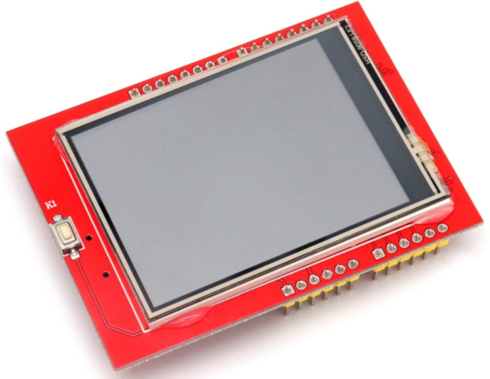
\includegraphics[scale=0.30]{figures/ili9341.png}
        \end{center}
        \caption{Lo schermo ILI9341.}
        \label{fig:ili9341}
    \end{subfigure}
    \hfill
    \begin{subfigure}[b]{0.45\textwidth}
        \begin{center}
            \begin{tikzpicture}[x=0.015cm, y=0.015cm, scale=0.65, transform shape]
                \draw   (120, 90) -- (320,90) -- (320,480) -- (120,480) -- cycle ;

\draw  [fill={rgb, 255:red, 255; green, 255; blue, 255 }  ,fill opacity=1 ]  (90,100)  --  (200,100) -- (200,130) --  (90,130) -- cycle;
\draw  [fill={rgb, 255:red, 255; green, 255; blue, 255 }  ,fill opacity=1 ]  (90,130)  --  (200,130) -- (200,160) --  (90,160) -- cycle;
\draw  [fill={rgb, 255:red, 255; green, 255; blue, 255 }  ,fill opacity=1 ]  (90,160)  --  (200,160) -- (200,190) --  (90,190) -- cycle;
\draw  [fill={rgb, 255:red, 255; green, 255; blue, 255 }  ,fill opacity=1 ]  (90,190)  --  (200,190) -- (200,220) --  (90,220) -- cycle;
\draw  [fill={rgb, 255:red, 255; green, 255; blue, 255 }  ,fill opacity=1 ]  (90,220)  --  (200,220) -- (200,250) --  (90,250) -- cycle;
\draw  [fill={rgb, 255:red, 255; green, 255; blue, 255 }  ,fill opacity=1 ]  (90,250)  --  (200,250) -- (200,280) --  (90,280) -- cycle;
\draw  [fill={rgb, 255:red, 255; green, 255; blue, 255 }  ,fill opacity=1 ]  (90,280)  --  (200,280) -- (200,310) --  (90,310) -- cycle;
\draw  [fill={rgb, 255:red, 255; green, 255; blue, 255 }  ,fill opacity=1 ]  (90,310)  --  (200,310) -- (200,340) --  (90,340) -- cycle;
\draw  [fill={rgb, 255:red, 255; green, 255; blue, 255 }  ,fill opacity=1 ]  (90,340)  --  (200,340) -- (200,370) --  (90,370) -- cycle;
\draw  [fill={rgb, 255:red, 255; green, 255; blue, 255 }  ,fill opacity=1 ]  (90,370)  --  (200,370) -- (200,400) --  (90,400) -- cycle;
\draw  [fill={rgb, 255:red, 255; green, 255; blue, 255 }  ,fill opacity=1 ]  (90,400)  --  (200,400) -- (200,430) --  (90,430) -- cycle;
\draw  [fill={rgb, 255:red, 255; green, 255; blue, 255 }  ,fill opacity=1 ]  (90,430)  --  (200,430) -- (200,460) --  (90,460) -- cycle;

\draw  [fill={rgb, 255:red, 255; green, 255; blue, 255 }  ,fill opacity=1 ] (250,100)  --  (380,100) -- (380,130) --  (250,130) -- cycle;
\draw  [fill={rgb, 255:red, 255; green, 255; blue, 255 }  ,fill opacity=1 ] (250,130)  --  (380,130) -- (380,160) --  (250,160) -- cycle;
\draw  [fill={rgb, 255:red, 255; green, 255; blue, 255 }  ,fill opacity=1 ] (250,160)  --  (380,160) -- (380,190) --  (250,190) -- cycle;
\draw  [fill={rgb, 255:red, 255; green, 255; blue, 255 }  ,fill opacity=1 ] (250,190)  --  (380,190) -- (380,220) --  (250,220) -- cycle;
\draw  [fill={rgb, 255:red, 255; green, 255; blue, 255 }  ,fill opacity=1 ] (250,220)  --  (380,220) -- (380,250) --  (250,250) -- cycle;
\draw  [fill={rgb, 255:red, 255; green, 255; blue, 255 }  ,fill opacity=1 ] (250,250)  --  (380,250) -- (380,280) --  (250,280) -- cycle;
\draw  [fill={rgb, 255:red, 255; green, 255; blue, 255 }  ,fill opacity=1 ] (250,280)  --  (380,280) -- (380,310) --  (250,310) -- cycle;
\draw  [fill={rgb, 255:red, 255; green, 255; blue, 255 }  ,fill opacity=1 ] (250,310)  --  (380,310) -- (380,340) --  (250,340) -- cycle;
\draw  [fill={rgb, 255:red, 255; green, 255; blue, 255 }  ,fill opacity=1 ] (250,340)  --  (380,340) -- (380,370) --  (250,370) -- cycle;


\draw (90,460) node [anchor=north west][inner sep=0.75pt]   [align=left] {$\displaystyle SD\_SCK$};
\draw (90,430) node [anchor=north west][inner sep=0.75pt]   [align=left] {$\displaystyle SD\_DO$};
\draw (90,400) node [anchor=north west][inner sep=0.75pt]   [align=left] {$\displaystyle SD\_DI$};
\draw (90,370) node [anchor=north west][inner sep=0.75pt]   [align=left] {$\displaystyle SD\_SS$};
\draw (90,340) node [anchor=north west][inner sep=0.75pt]   [align=left] {$\displaystyle LCD\_D1$};
\draw (90,310) node [anchor=north west][inner sep=0.75pt]   [align=left] {$\displaystyle LCD\_D0$};
\draw (90,280) node [anchor=north west][inner sep=0.75pt]   [align=left] {$\displaystyle LCD\_D7$};
\draw (90,250) node [anchor=north west][inner sep=0.75pt]   [align=left] {$\displaystyle LCD\_D6$};
\draw (90,220) node [anchor=north west][inner sep=0.75pt]   [align=left] {$\displaystyle LCD\_D4$};
\draw (90,190) node [anchor=north west][inner sep=0.75pt]   [align=left] {$\displaystyle LCD\_D5$};
\draw (90,160) node [anchor=north west][inner sep=0.75pt]   [align=left] {$\displaystyle LCD\_D3$};
\draw (90,130) node [anchor=north west][inner sep=0.75pt]   [align=left] {$\displaystyle LCD\_D2$};

\draw (250,370) node [anchor=north west][inner sep=0.75pt]   [align=left] {$\displaystyle 3.3V$};
\draw (250,340) node [anchor=north west][inner sep=0.75pt]   [align=left] {$\displaystyle 5V$};
\draw (250,310) node [anchor=north west][inner sep=0.75pt]   [align=left] {$\displaystyle GND$};
\draw (250,280) node [anchor=north west][inner sep=0.75pt]   [align=left] {$\displaystyle LCD\_RD$};
\draw (250,250) node [anchor=north west][inner sep=0.75pt]   [align=left] {$\displaystyle LCD\_WR$};
\draw (250,220) node [anchor=north west][inner sep=0.75pt]   [align=left] {$\displaystyle LCD\_RS$};
\draw (250,190) node [anchor=north west][inner sep=0.75pt]   [align=left] {$\displaystyle LCD\_CS$};
\draw (250,160) node [anchor=north west][inner sep=0.75pt]   [align=left] {$\displaystyle LCD\_RST$};
\draw (250,130) node [anchor=north west][inner sep=0.75pt]   [align=left] {$\displaystyle F\_CS$};

            \end{tikzpicture}
        \end{center}
        \caption{Pinout dello schermo \texttt{ILI9341}.}
        \label{fig:pinout_ili}
    \end{subfigure}
\end{figure}

Per quanto riguarda lo schermo dell'emulatore abbiamo optato per un display TFT LCD
a colori retroilluminato (Fig. \ref{fig:ili9341}) basato sul controller \texttt{ILI9341}.
Il display ha una dimensione di 2.4 pollici, una risoluzione di 320$\times$240\texttt{px} e
al suo interno è presente un lettore di schede microSD integrato.

\begin{figure}[h!t]
    \begin{subfigure}[b]{0.45\textwidth}
        \begin{center}
            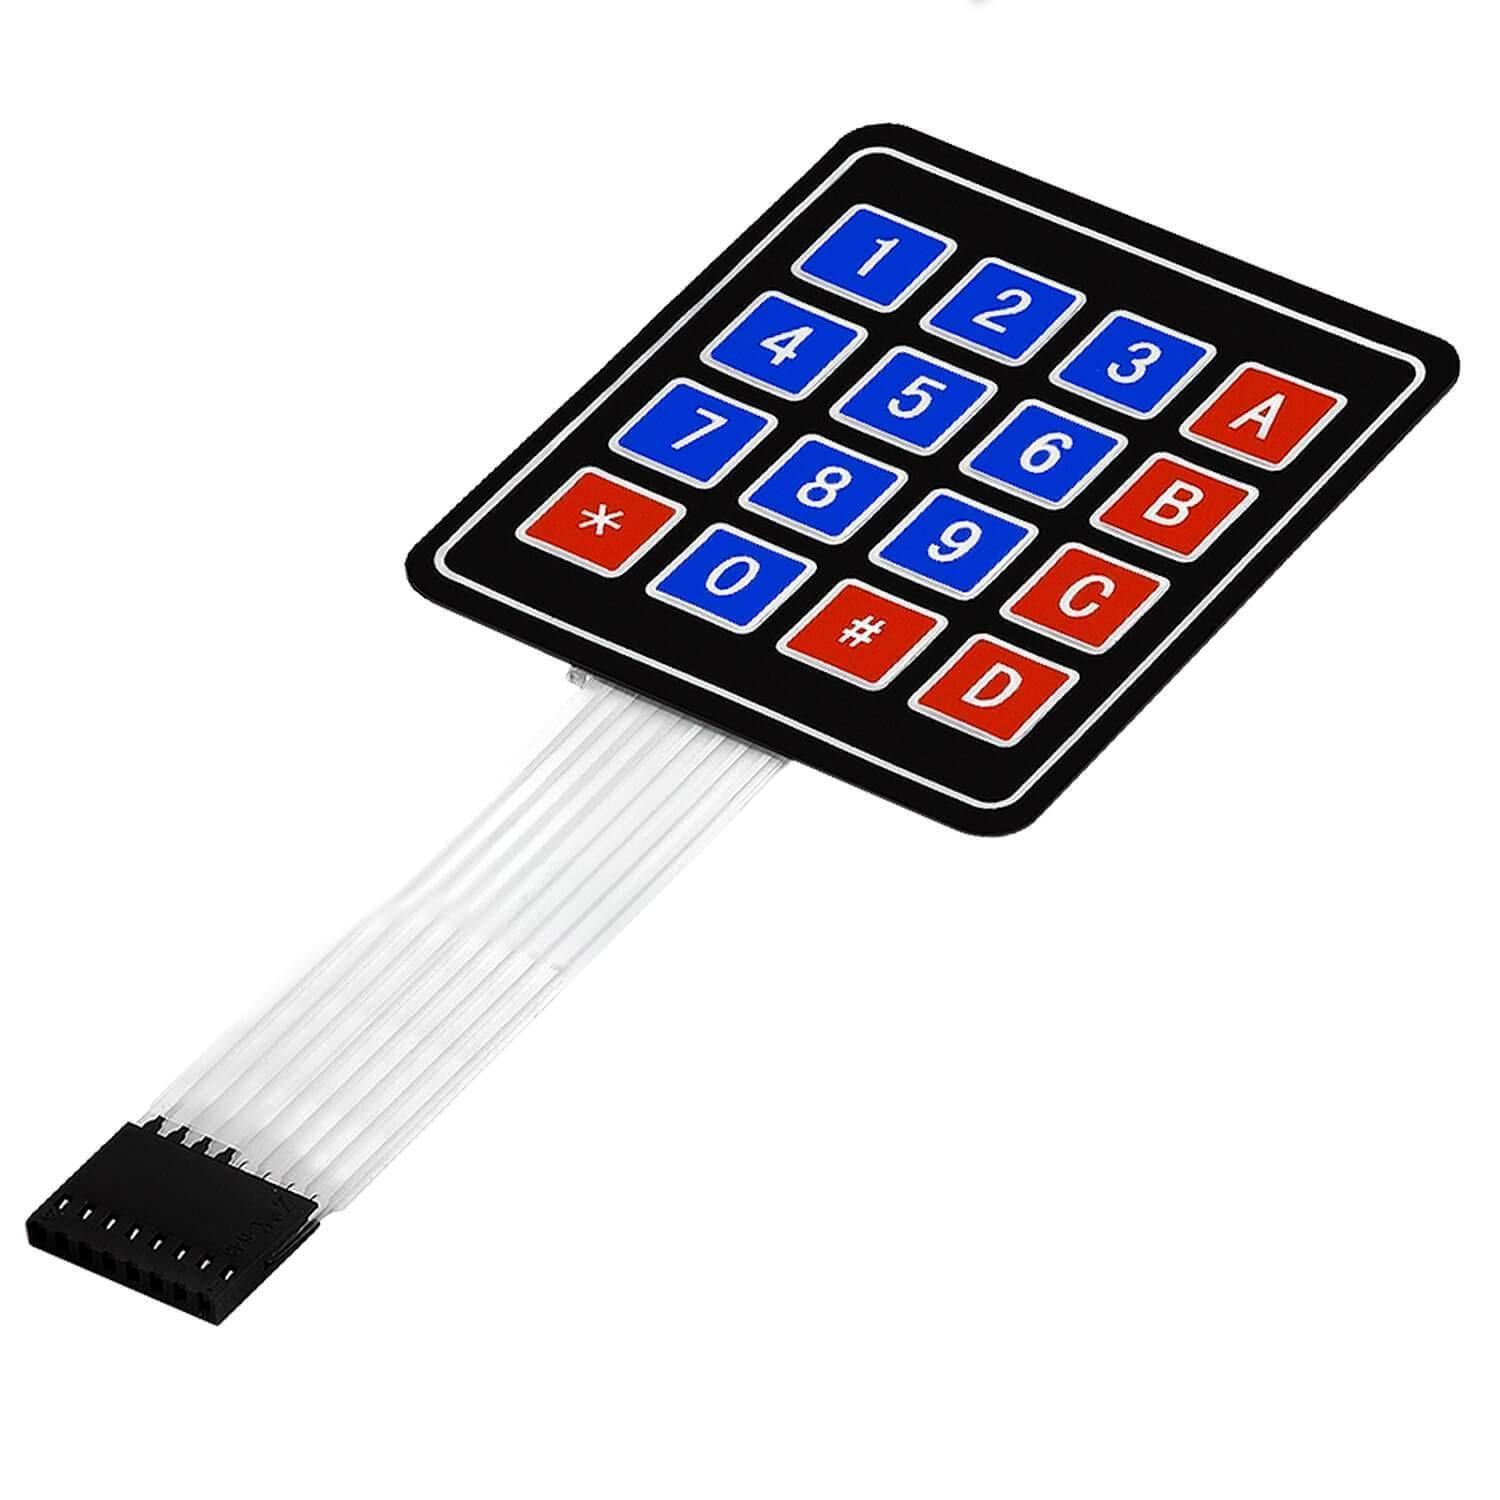
\includegraphics[scale=0.090]{figures/4x4_keypad.jpeg}
        \end{center}
        \caption{Il tastierino matriciale 4$\times$4.}
        \label{fig:4x4_keypad}
    \end{subfigure}
    \hfill
    \begin{subfigure}[b]{0.45\textwidth}
        \begin{center}
            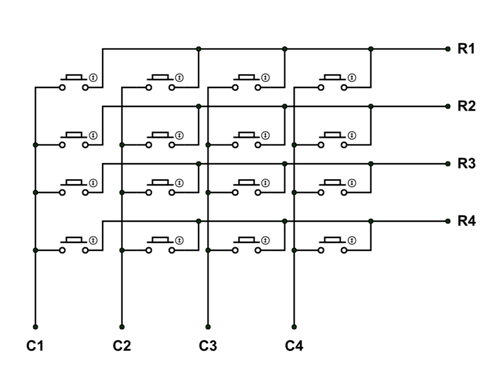
\includegraphics[scale=0.30]{figures/4x4_keypad_structure.png}
        \end{center}
        \caption{Struttura del tastierino matriciale 4$\times$4.}
        \label{fig:4x4_keypad_structure}
    \end{subfigure}
\end{figure}

Per poter interagire con l'emulatore abbiamo utilizzato un tastierino matriciale 4$\times$4
(Fig. \ref{fig:4x4_keypad}) analogo alla tastiera originale del
COSMAC VIP\footnote{https://en.wikipedia.org/wiki/COSMAC\_VIP}, un microcomputer
creato da Joseph Weisbecker appositamente per CHIP-8.

Infine, per supportare gli effetti sonori riprodotti dai videogiochi CHIP-8 abbiamo
utilizzato un beeper passivo monotono, che anche essendo un dispositivo molto semplice
adempie correttamente ai suoi compiti dato che il suono prodotto da un emulatore CHIP-8
deve avere solo un tono.

\subsection{Componenti utilizzati e relativi costi}

\begin{table}[h!t] % [ht]
    \centering
    \begin{tabular}{|llll|l|}
        \hline
        \multicolumn{1}{|l|}{\textbf{Descrizione}}          & \multicolumn{1}{l|}{\textbf{Modello}}       & \multicolumn{1}{l|}{\textbf{Costo unitario}} & \textbf{Unità} & \textbf{Costo} \\ \hline
        \multicolumn{1}{|l|}{Microcontrollore}       & \multicolumn{1}{l|}{STM32 F334R8T6}         & \multicolumn{1}{l|}{14.99}                   & 1               & 14.99          \\ \hline
        \multicolumn{1}{|l|}{Schermo}                & \multicolumn{1}{l|}{ILI9341 2.4"}           & \multicolumn{1}{l|}{6.50}                    & 1               & 6.50           \\ \hline
        \multicolumn{1}{|l|}{Tastierino}          & \multicolumn{1}{l|}{Matrix keypad 4$\times$4} & \multicolumn{1}{l|}{3.99}                    & 1               & 3.99           \\ \hline
        \multicolumn{1}{|l|}{Beeper}                 & \multicolumn{1}{l|}{}                       & \multicolumn{1}{l|}{0.99}                    & 1               & 0.99           \\ \hline
        \multicolumn{1}{|l|}{Cablaggio} & \multicolumn{1}{l|}{}                       & \multicolumn{1}{l|}{4.99}                    & 1               & 4.99           \\ \hline
        \multicolumn{1}{|l|}{Interruttore e altri materiali} & \multicolumn{1}{l|}{}       & \multicolumn{1}{l|}{4.99}                    & 1               & 4.99           \\ \hline
        \multicolumn{1}{|l|}{Scocca} & \multicolumn{1}{l|}{GW42002}                       & \multicolumn{1}{l|}{9.99}                    & 1               & 9.99           \\ \hline
        \multicolumn{4}{|r|}{\textbf{Totale}}                                                      & 46.50\euro    \\ \hline
    \end{tabular}
    \caption{
        Materiali utilizzati per la realizzazione del progetto.
    }
    \label{tab:components}
\end{table}

In Tabella \ref{tab:components} è possibile vedere i componenti utilizzati per la
realizzazione del progetto. I costi indicati provengono da negozi online come Amazon e eBay.

\subsection{Schema di collegamento}

\textbf{Legenda dei colori in Figura \ref{fig:schema}}

\begin{itemize}
    \item \textcolor{green}{Verde}: Schermo
    \item \textcolor{blue}{Blu}: Scheda microSD
    \item \textcolor{magenta}{Magenta}: Tastierino
    \item \textcolor{orange}{Arancione}: Beeper
    \item \textcolor{cyan}{Ciano}: Reset
    \item \textcolor{black}{Nero}: GND
    \item \textcolor{red}{Rosso}: Alimentazione
\end{itemize}

\begin{figure}[h!t]
    \begin{center}
        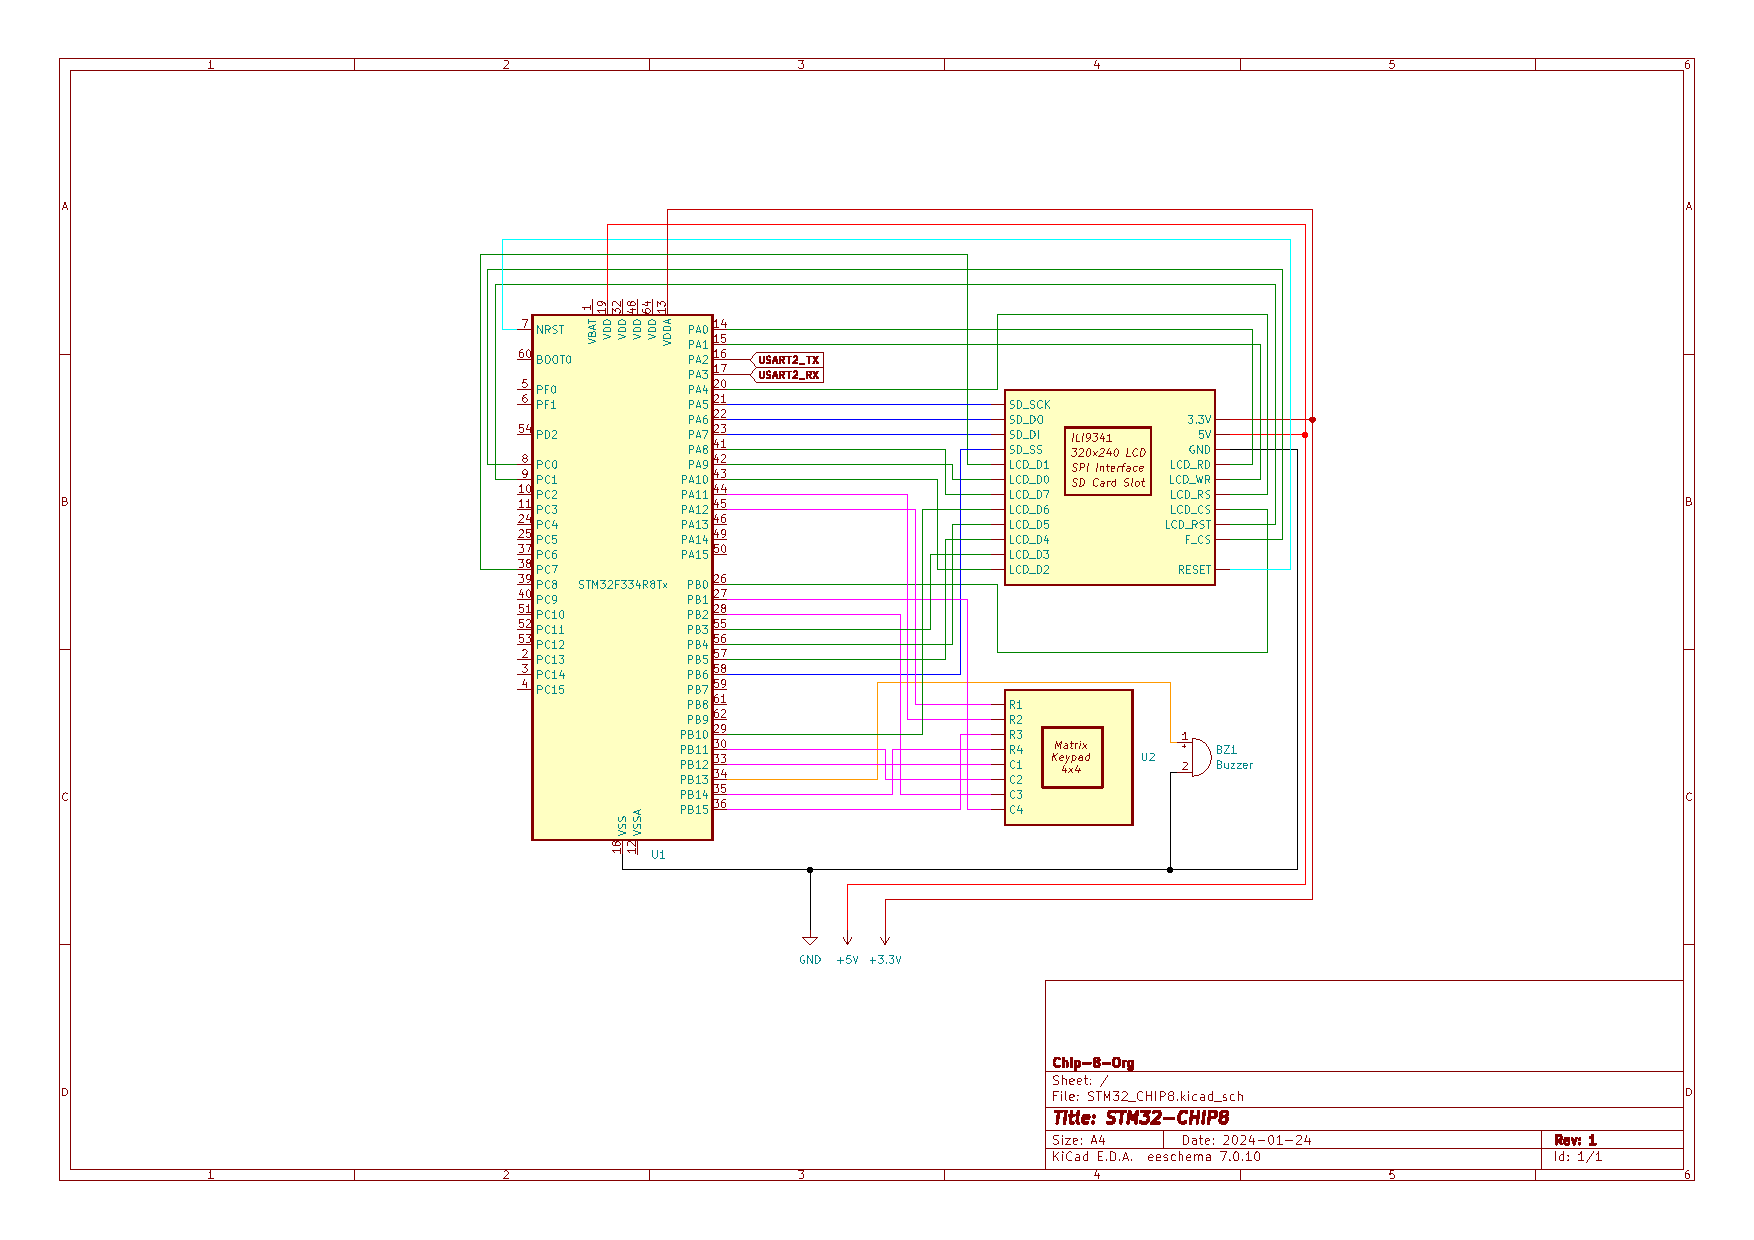
\includegraphics[scale=0.50]{figures/STM32_CHIP8.pdf}
    \end{center}
    \caption{
        Schema del progetto.
    }
    \label{fig:schema}
\end{figure}

\subsubsection{Schema di collegamento}\label{subsubsec:collegamenti}

In Figura \ref{fig:schema} è possibile vedere lo schema di collegamento
dei componenti hardware realizzato utilizzando il software \texttt{KiCad}.
Il display e il lettore microSD integrato sono stati collegati al microcontrollore
attraverso il pinout standard degli Shields di Arduino, un'interfaccia hardware che permette
di collegare una scheda Arduino ad un modulo esterno.

Il tastierino matriciale 4$\times$4 è stato collegato al microcontrollore tramite 8 pin GPIO.
In particolare i 4 pin relativi alle righe (\texttt{R1}, \texttt{R2}, \texttt{R3}, \texttt{R4})
sono stati impostati in modalità \texttt{GPIO\_MODE\_IT\_RISING} (interrupt rising edge).

Quando un pin GPIO viene configurato come sorgente di interrupt sul fronte di salita
il segnale di interrupt è generato quando il pin passa da basso (0) ad alto (1), risultando
particolarmente utile per intercettare il cambiamento dello stato di un
pulsante quando viene premuto.

Invece, i 4 pin relativi alle colonne (\texttt{C1}, \texttt{C2}, \texttt{C3}, \texttt{C4})
sono stati impostati in modalità \texttt{GPIO\_MODE\_OUTPUT\_PP} (push-pull output) per
consentire l'invio dell'interrupt alla pressione di un tasto, dato che chiudendo il circuito
si permette alla corrente proveniente dal pin GPIO di fluire verso i pin di interrupt.
Successivamente viene identificato il tasto premuto, questo meccanismo verrà elaborato
nella sezione \ref{subsubsec:keypad}.

Infine, il beeper è stato collegato al microcontrollore tramite un pin GPIO e GND.
Quest'ultimo è stato impostato in modalità \texttt{GPIO\_MODE\_OUTPUT\_PP} (push-pull output)
per permettere l'invio di un segnale al beeper.

\section{Software}

Il nostro software si divide in due componenti principali: l'interprete CHIP-8 e
l'infrastruttura necessaria per "portarlo" sul microcontrollore STM32, ovvero l'interfaccia
con lo schermo e i gestori per la scheda microSD, per il keypad e per il beeper.

\subsection{Interprete CHIP-8}

\begin{Listing}[h!t] % [ht]
    \centering
    \showc*[.8\textwidth]{chip8_struct.c}
    \caption{La struttura che rappresenta lo stato della macchina virtuale}
    \label{chip8_struct}
\end{Listing}

Abbiamo deciso di scrivere l'interprete da zero e per farlo è stato necessario consultare
le specifiche (de facto standard) che definiscono il comportamento di un interprete CHIP-8
\cite{cowgod:chip8} e S-CHIP \cite{cowgod:schip}.

L'interprete ha un'architettura basata su registri e possiede 4 KB di memoria, 16 registri
general purpose, un registro per gli indirizzi di memoria, un registro per il delay timer,
un registro per il sound timer, uno stack per gestire le chiamate a subroutine, uno stack pointer
e un program counter.

Il delay timer viene utilizzato come cronometro mentre il sound
timer è utilizzato per gestire gli effetti sonori, quando il suo
valore è diverso da zero, l'emulatore attiva il beeper.

Ad ogni ciclo di esecuzione l'interprete effettua il fetch
dell'istruzione puntata dal program counter in memoria,
la decodifica e la esegue.

Sono supportate 45 istruzioni diverse, ciascuna delle
quali è rappresentata da uno specifico opcode in cui al suo interno
sono passati anche eventuali parametri.

Il programma è scritto in C99, non ha I/O ed è freestanding
\cite{n1256:conformance}, ovvero non dipende dalla libreria
standard del C (libc). Tutto questo è mirato a rendere l'interprete
altamente portabile.

Per rimuovere la dipendenza da libc è stato necessario includere
alcune funzioni direttamente da libgcc, trovare un modo alternativo
per implementare le asserzioni e includere una funzione ad hoc per
la generazione di numeri casuali.

% TODO - spiegare il codice

\begin{Listing}[h!t]
    \centering
    \mbox{
        \showc[.45\textwidth]{assert.c}
        \quad
        \showc[.50\textwidth]{random.c}
    }
    \caption{Implementazioni di \texttt{ASSERT} e \texttt{rand\_byte}.}
    \label{assert_rand}
\end{Listing}

Infine per testare più comodamente l'interprete abbiamo sviluppato
un semplice emulatore su desktop utilizzando SDL2
\cite{libsdl:about}, una libreria scritta in C che consente di
gestire audio, video e input da tastiera.
In seguito l'interprete è stato sottoposto ad un'apposita
test suite \cite{github:chip8-test-suite} che mira a verificare
il comportamento corretto di ciascun opcode.

\subsubsection{Gestione del timing}

Uno dei problemi principali durante lo sviluppo di un emulatore è
la gestione del timing, in particolare è necessario limitare la
"velocità" dell'emulatore bloccando temporaneamente la sua
esecuzione.

Inoltre abbiamo dovuto disaccoppiare la frequenza dell'interprete
(regolabile dal giocatore) dalla frequenza del delay timer e del
sound timer (costante a 60 Hz). Dove con frequenza dell'interprete
ci riferiamo al numero di istruzioni che esegue ogni frame.

% TODO - "durante lo sviluppo abbiamo testato due soluzioni diverse"

Inizialmente abbiamo optato per la gestione di una singola istruzione per ciclo di esecuzione,
di conseguenza il ritardo del game loop risultava variabile e dipendeva dalla frequenza selezionata
dal giocatore. Per assicurare una frequenza $\mathcal{F}$ di 60 Hz i timer venivano decrementati
ogni n-esima iterazione del game loop, dove $n = \frac{\mathcal{F}}{60}$. Ad esempio se
$\mathcal{F} = 540$, i timer venivano decrementati ogni $9^{\circ}$ ciclo.

Purtroppo però questo approccio presenta un problema non trascurabile, ovvero effettua una chiamata
ad una funzione simil-sleep per un periodo molto breve dopo ogni istruzione. Ad esempio se
$\mathcal{F} = 540$, il ritardo di una sleep sarebbe solo di 1.85 ms, e questo genere di funzione
non offre una precisione simile. Per questo motivo abbiamo optato per una soluzione differente.

Abbiamo fissato il ritardo del game loop a 16.666 ms, un valore sufficientemente alto da non avere
problemi di granularità. Inoltre in questo modo otteniamo un frame rate di 60 fps esatti.
Avendo reso il ritardo costante abbiamo dovuto rendere variabile il numero di istruzioni gestite
durante un ciclo di esecuzione. In particolare vengono gestite n istruzioni per ciclo,
dove $n = \frac{\mathcal{F}}{60}$. Ad esempio se $\mathcal{F} = 540$, vengono gestite 9 istruzioni
per ciclo. A questo punto dato che il game loop viene ripetuto con una frequenza di 60 Hz risulta
banale gestire la frequenza dei timer.

Sono state considerate anche eventuali problematiche che sarebbero potute sorgere con questo
approccio. In particolare non tutte le istruzioni impiegano lo stesso tempo per essere eseguite,
ma fortunatamente anche l'istruzione più lenta richiede una quantità trascurabile di tempo.
Ciò significa che possiamo comportarci come se tutte le istruzioni richiedessero il medesimo tempo.

\subsubsection{Ottimizzazioni}

\begin{figure}[h!t]
    \begin{center}
        % 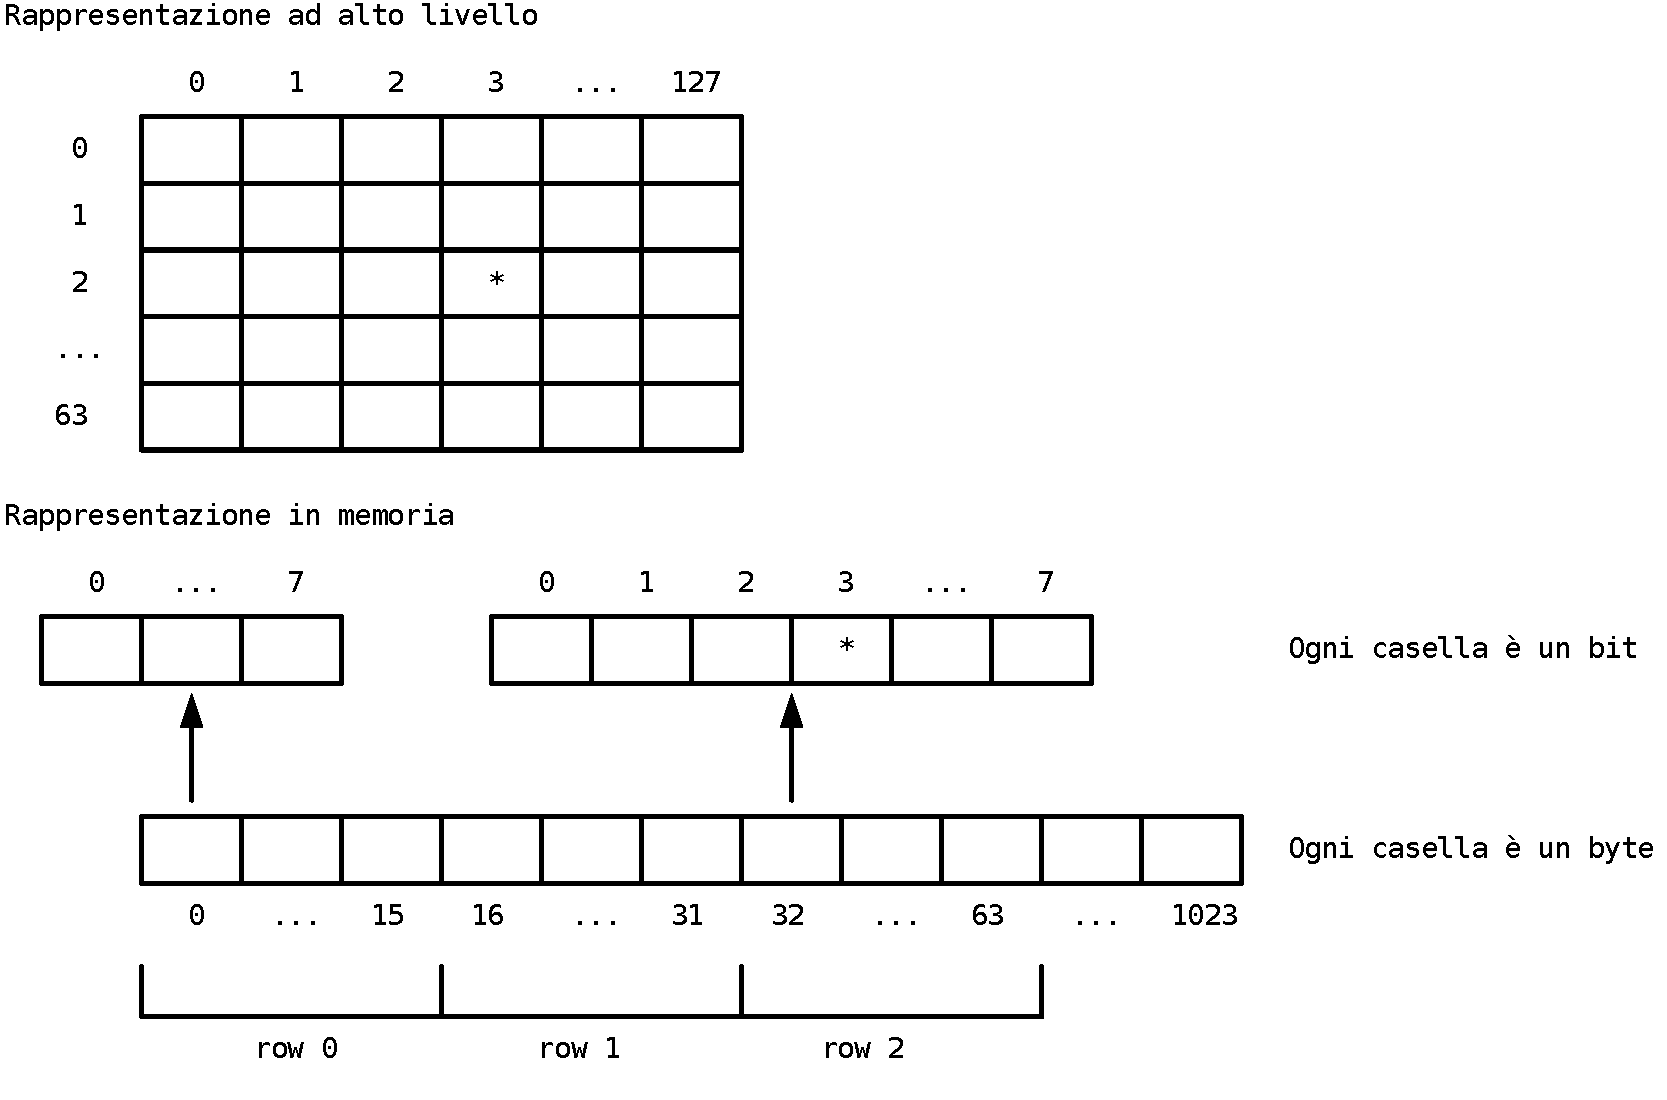
\includegraphics[scale=0.3]{figures/screenopt.pdf}
        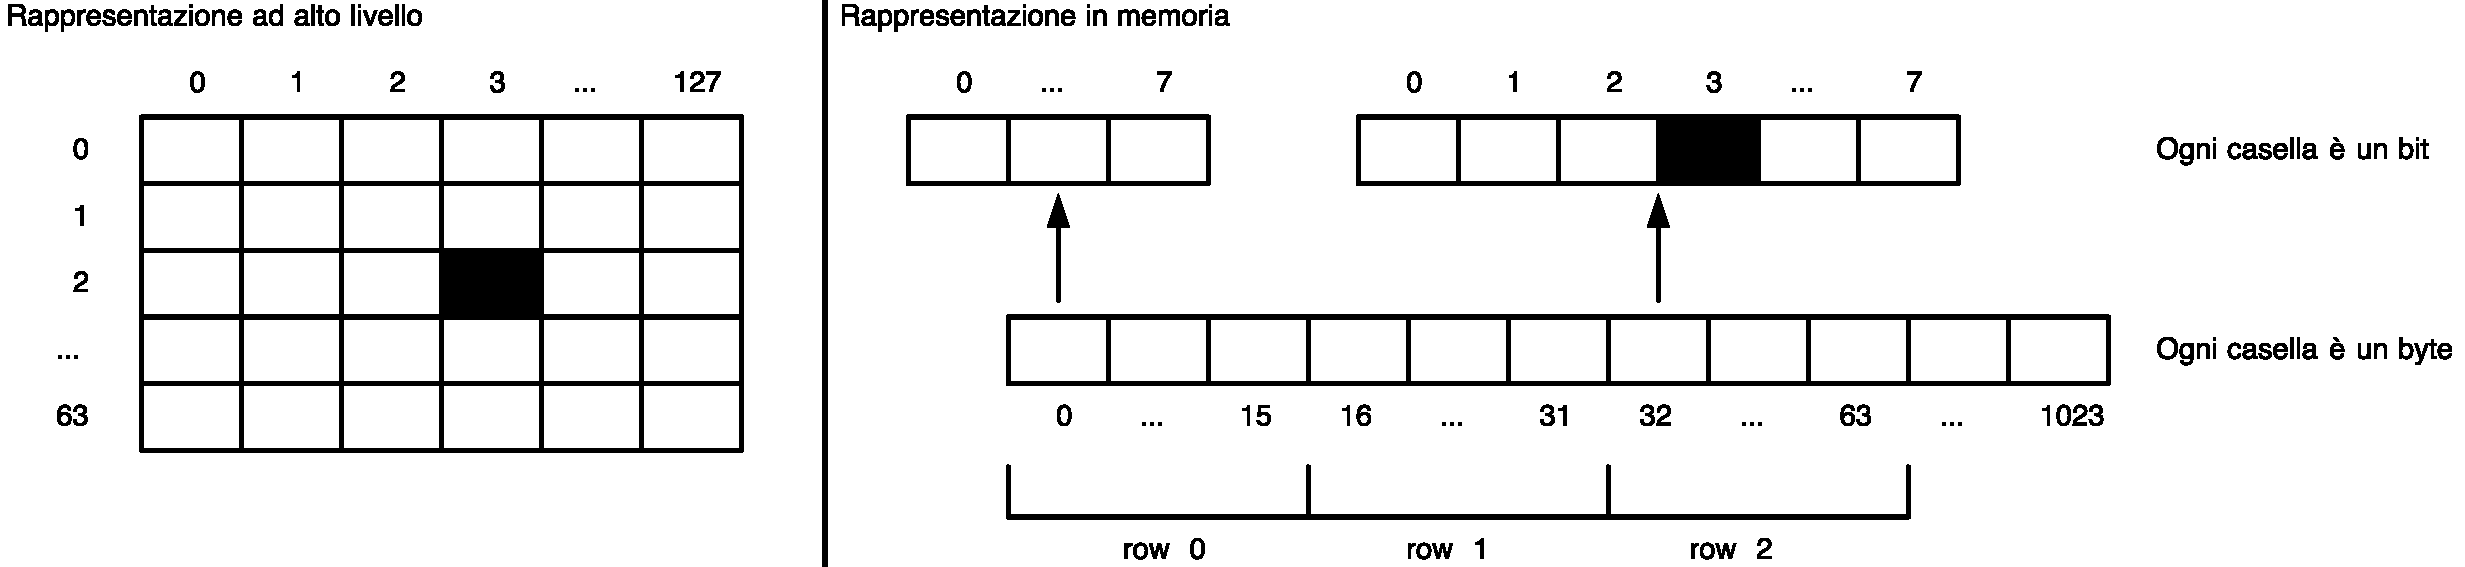
\includegraphics[scale=0.38]{figures/screenopt_small.pdf}
    \end{center}
    \caption{Esempio della mappatura di un pixel.}
    \label{fig:screenopt}
\end{figure}

È stato necessario introdurre delle ottimizzazioni all'interno
dell'interprete per poterlo far girare su un microcontrollore.

L'ottimizzazione principale è legata alla rappresentazione dello
schermo in memoria. Ad alto livello lo schermo può essere visto
come una matrice di 128x64 pixel monocromi. Una rappresentazione
simile occuperebbe 8192 byte, dato che ciascun pixel verrebbe
rappresentato da un byte.

Purtroppo il nostro microcontrollore ha a disposizione solamente 16 KB di SRAM, di conseguenza
una soluzione simile non è praticabile.

Per questo motivo abbiamo deciso di rappresentare lo schermo come un array unidimensionale di
1024 byte, dove ciascun pixel viene rappresentato da un singolo bit. In questo modo otteniamo
un risparmio di spazio pari a ben l'87.5\%.

Questa decisione ha aggiunto però un livello di indirezione dato
che una coordinata ad alto livello sulla matrice 128x64 deve essere
mappata ad una coordinata "in memoria".

Un'ulteriore ottimizzazione viene resa disponibile attraverso l'API
dell'interprete sotto forma di una funzione che consente al chiamante
di controllare se l'array che rappresenta lo schermo è stato
modificato nell'ultimo ciclo di esecuzione. In questo modo la grafica
viene renderizzata dal chiamante solo quando è effettivamente
necessario.

\subsubsection{Comportamenti ambigui}

Gli interpreti CHIP-8 e S-CHIP hanno sviluppato molteplici
comportamenti ambigui nel corso degli anni. Questi cosiddetti
"quirk" variano in base alle piattaforme per cui è stato sviluppato
l'interprete. Ad esempio gli interpreti per calcolatrici HP 48
presentano un comportamento leggermente diverso durante l'esecuzione
delle istruzioni di SHIFT.

Questi comportamenti ambigui si propagano fino ai programmatori
CHIP-8 che si appoggiano a quest'ultimi e scrivono videogiochi che
non sono del tutto compatibili con interpreti più vecchi. Per evitare
questa frammentazione è necessario supportare le piattaforme
principali e i loro quirk.

Il nostro interprete supporta CHIP-8, CHIP-48, S-CHIP 1.0 e
S-CHIP 1.1, in questo modo è in grado di eseguire la stragrande
maggioranza dei videogiochi reperibili in rete.

\subsection{Porting su STM32}

Dopo aver terminato l'interprete abbiamo sviluppato un'infrastruttura per poterlo eseguire
sul microcontrollore STM32.

Come già anticipato, l'infrastruttura si compone di un'interfaccia con lo schermo,
un gestore per la scheda microSD, un gestore per il tastierino e un gestore per il beeper.

È importante ricordare che l'interprete è stato progettato per essere altamente portabile
e indipendente dalla piattaforma su cui verrà eseguito, per questo motivo non è stato necessario
apportare modifiche significative.

Tuttavia, a causa della potenza limitata della scheda la fluidità del gameplay è inferiore
rispetto alla port su SDL2 che viene eseguita su normale computer.

\subsubsection{Architettura software}

\begin{figure}[h!t]
    \begin{center}
        \begin{tikzpicture}[scale=0.6, transform shape]
            \renewcommand{\umltextcolor}{black}
\renewcommand{\umldrawcolor}{black}
\renewcommand{\umlfillcolor}{white}

  \begin{class}[text width=2cm]{Main}{6,0}
    \operation{+ main()}
  \end{class}

  \begin{class}[text width=3cm]{Keypad}{0,-2}
      \operation{+ interrupt()}
      \operation{+ \sout{polling()}}
  \end{class}

  \begin{class}[text width=1.7cm]{Chip8}{3,-3}
    \operation{+ init()}
    \operation{+ cylce()}
    \operation{+ ended()}
  \end{class}


  \begin{class}[text width=3.5cm]{ILI9341}{6, -4}
    \operation{+ init(\texttt{Pin[13]})}
    \operation{+ drawMenu(\texttt{char*[]})}
    \operation{+ fillScreen(\texttt{uint16\_t})}
    \operation{+ drawGame(\texttt{char[]})}
  \end{class}

  \begin{class}[text width=1.7cm]{Beeper}{9,-3}
      \operation{+ high()}
      \operation{+ low()}
  \end{class}

  \begin{class}[text width=3cm]{SD}{12, -2}
    \operation{+ mount()}
    \operation{+ open()}
    \operation{+ read()}
    \operation{+ readFile(\texttt{char[]})}
    \operation{+ close()}
  \end{class}

  % \begin{class}[text width=2.4cm]{Menu}{10,0}
  %     \operation{+ loadGame()}
  % \end{class}

    % \draw [umlcd style dashed line , ->] (Menu) -- node [ above , sloped , black ]{} (Keypad) ;
    % \draw [umlcd style dashed line , ->] (Menu) -- node [ above , sloped , black ]{} (SD) ;
    % \draw [umlcd style dashed line , fill=white, ->] (Menu) -- node [ below  , black ]{} (ILI9341) ;

    % \draw [umlcd style dashed line , ->] (Main) -- node [ above , sloped , black ]{} (Menu) ;
    \draw [umlcd style dashed line , ->] (Main) -- node [ above , sloped , black ]{} (Chip8) ;
    \draw [umlcd style dashed line , ->] (Main) -- node [ above , sloped , black ]{} (Keypad) ;
    \draw [umlcd style dashed line , ->] (Main) -- node [ above , sloped , black ]{} (Beeper) ;
    \draw [umlcd style dashed line , fill=white, ->] (Main) -- node [ below , sloped , black ]{} (SD) ;
    \draw [umlcd style dashed line , fill=white, ->] (Main) -- node [ below , sloped , black ]{} (ILI9341) ;

    \begin{scope}[xshift=0cm, yshift=0cm] % Adjust the positioning of the legend
    % Legend title
    \node[font=\bfseries] at (0, 0) {Legend};
    % Legend items
    \draw [umlcd style dashed line , fill=white, ->] (0, -0.5) -- (1, -0.5) node[right,  black] {Uses};
    \end{scope}

  % \draw [ umlcd style , ->] (Main) -- node [ above , sloped , black ]{$ < <$ import $ > >$} (Student) ;

        \end{tikzpicture}
    \end{center}
    \caption{
       Class diagram.
    }
    \label{fig:class_diagram}
\end{figure}

In Figura \label{fig:class_diagram} è rappresentato il class diagram, il quale offre una panoramica
dell'architettura del software. Una differenza da evidenziare rispetto alla proposta iniziale
è che la classe \texttt{menù} non è più presente perché è stata integrata all'interno della
classe \texttt{main}.

\begin{figure}[h!t]
    \begin{center}
        \resizebox{0.6\textwidth}{!}{%
        \begin{sequencediagram}
        \newthread{main}{:Main}
        % \newinst[0.5]{menu}{:Menu}
        \newinst[0.5]{vm}{:Chip8}
        \newinst[0.5]{lcd}{:ILI9341}
        \newinst[0.5]{kp}{:Keypad}
        \newinst[0.5]{beep}{:Beeper}
        \newinst[0.5]{sd}{:SD}

        \begin{call}{main}{mount(); open(); read();}{sd}{}
        \end{call}
        \begin{sdblock}{Game Selection Loop (Menu)}{}
            \begin{call}{main}{interrupt()}{kp}{}
            \end{call}
            \begin{call}{main}{drawMenu(\texttt{char*[]})}{lcd}{}
            \end{call}
        \end{sdblock}
        \begin{call}{main}{readFile(\texttt{char[]})}{sd}{}
        \end{call}

        \begin{call}{main}{init()}{vm}{}
        \end{call}

        \begin{sdblock}{Main Loop}{}
            \begin{call}{main}{interrupt()}{kp}{}
            \end{call}
            \begin{call}{main}{cycle()}{vm}{}
            \end{call}
            \begin{call}{main}{high() / low()}{beep}{}
            \end{call}
            \begin{call}{main}{drawGame(\texttt{char[]})}{lcd}{}
            \end{call}
        \end{sdblock}
        \end{sequencediagram}
    }

    \end{center}
    \caption{
        Sequence diagram.
    }
    \label{fig:sequence_diagram}
\end{figure}

Il flusso di esecuzione dell'emulatore è mostrato in Figura \ref{fig:sequence_diagram},
per prima cosa vengono letti i nomi dei file presenti sulla scheda microSD, in seguito
si entra nel game selection loop dove il giocatore potrà selezionare un gioco, la velocità
dell'interprete e la piattaforma da emulare. Una volta selezionato il gioco si entrerà nel
game loop dove inizia la fase di emulazione vera e propria.

\subsubsection{Interfaccia con la scheda microSD}\label{subsubsec:sd}

La scheda microSD è utilizzata come memoria di massa dell'emulatore contenente i file
binari dei videogiochi CHIP-8. È stata formattata con FAT32 e viene gestita utilizzando
\texttt{FatFs} \cite{elm-chan:fatfs}, una libreria open source che permette di
interfacciarsi con questa tipologia di filesystem.

La comunicazione tra il microcontrollore e la scheda microSD avviene tramite il protocollo
\textit{Serial Peripheral Interface} (SPI), dove il microcontrollore è configurato come
master e la scheda microSD come slave.

% FIXME - non è una considerazione un po' random messa così?
%
% A differenza di altri protocolli come l'I2C, che fanno uso di indirizzi per identificare
% dispositivi sulla stessa linea di comunicazione, SPI non li utilizza. Tuttavia,
% SPI rimane un'opzione valida e popolare per la comunicazione su bus nei sistemi embedded.

% FIXME
%
% Abbiamo effettuato una piccola ottimizzazione decidendo di non abilitare
% il Long File Names (LFN) sul filesystem FAT32 della scheda microSD.
% Questo implica il fatto che tutti i file devono avere un nome di al massimo 13 byte
% (caratteri ASCII). Cosi' facendo abbiamo risparmiato in termini complessità di computazione,
% memoria flash e SRAM.

\subsubsection{Menù di selezione}

La selezione del gioco avviene tramite un apposito menù che lista su più pagine tutti i giochi
presenti sulla scheda microSD. Per aggiungere un gioco è sufficiente caricarlo sulla scheda
microSD e riavviare il microcontrollore, poiché il menu viene generato dinamicamente.
Inoltre, il menù permette anche di impostare la velocità e la modalità di esecuzione
dell'interprete.

L'utente interagisce con il menù attraverso il tastierino, in particolare abbiamo predisposto
dei tasti riservati per la navigazione tra le pagine, per la selezione della velocità e
della modalità di esecuzione. I tasti rimanenti vengono utilizzati per avviare specifici giochi.

Infine, per risolvere il problema degli artefatti grafici al cambio di schermata,
abbiamo implementato una funzione dedicata per "pulire" lo schermo e ottenere un effetto
di transizione da una schermata all'altra.

% TODO
\subsubsection{Funzionamento del keypad}\label{subsubsec:keypad}

Inizialmente il keypad è stato gestito tramite polling, ovvero il microcontrollore controllava
ad ogni aggiornamento dello schermo (60 \texttt{FPS} $\approx$ 16.666 ms) lo stato dei pin di riga
e di colonna per capire quale tasto fosse stato premuto. Questo approccio è stato scartato in
favore dell'approccio basato su interrupt, in quanto il polling consumava molte risorse del
microcontrollore e non garantiva un framerate stabile in quanto in $\sim$16 ms non riusciva a
garantire la lettura di tutti i pin ed eseguire le restanti operazioni.

La procedura di gestione degli interrupt su microcontrollori STM32 è standard. Bisogna implementare
una funzione che gestisce l'interrupt e bisogna configurare il pin GPIO come sorgente di interrupt.
Nel nostra situazione, come accennato in sezione \ref{subsubsec:collegamenti}, i pin di riga sono
stati impostati in modalità \texttt{GPIO\_MODE\_IT\_RISING} (interrupt rising edge) e i pin di
colonna in modalità \texttt{GPIO\_MODE\_OUTPUT\_PP} (push-pull output) per permettere l'invio
dell'interrupt alla pressione di un tasto.

Successivamente, viene capito quale tasto è stato premuto, leggendo il valore dei pin
di riga e di colonna. Per fare ciò, i pin di riga sono stati impostati in modalità
\texttt{GPIO\_MODE\_INPUT}. Come si può vedere nel listato \ref{keypad} a riga 1,
nella routine di interrupt viene abilitato il pin di output della prima colonna e in seguito
per ogni riga viene letto il valore del pin di input per conoscere la seconda coordinata
del tasto premuto, e in caso sia premuto viene salvato nella struttura dati apposita
nella macchina virtuale. Questa operazione viene ripetuta per ognuna delle quattro colonne.
Al termine della routine di interrupt
({\setmintedinline[c]{style=friendly}\inlinec{void Interrupt_handle_keypad(uint16_t GPIO_Pin)}}),
i pin di riga vengono re-impostati in modalità \texttt{GPIO\_MODE\_IT\_RISING} per permettere
l'invio dell'interrupt alla pressione di un nuovo tasto.

\begin{Listing}[h!t] % [ht]
    \centering
    \setminted[c]{escapeinside=@@}
    \showc*[.87\textwidth]{keypad.c}
    \caption{Gestione dell'interrupt del keypad.}
    \label{keypad}
\end{Listing}

% TODO
\subsubsection{Interfaccia con lo schermo}

Il driver per display a cristalli liquidi \texttt{ILI9341} consente la comunicazione tramite due
diverse interfacce: SPI (spiegata in sezione \ref{subsubsec:sd}) e 8 bit parallela. Mentre
l'interfaccia SPI richiede meno pin, è più lenta a causa del protocollo seriale. Al contrario,
l'interfaccia parallela è più veloce ma richiede più pin. Poiché dobbiamo visualizzare
i videogiochi sullo schermo e aggiornare l'immagine a circa 60 volte al secondo, abbiamo
optato per l'interfaccia parallela.

L'interfaccia parallela è un metodo di comunicazione che coinvolge l'invio simultaneo di più
bit di dati attraverso una serie di linee di comunicazione parallele. Nel contesto del display
LCD ILI9341, l'interfaccia parallela ad 8 bit coinvolge l'uso di otto linee di dati per
trasmettere informazioni al display. Oltre alle linee di dati, ci possono essere anche altre
linee di controllo, come quelle per il segnale di sincronizzazione e i segnali di controllo.
Quando si utilizza l'interfaccia parallela, i dati vengono inviati al display in gruppi di 8 bit
simultaneamente, consentendo un trasferimento più rapido rispetto all'interfaccia SPI,
che invia i dati bit per bit in sequenza.

Per l'inizializzazione abbiamo utilizzato la funzione
{\setmintedinline[c]{style=friendly}\inlinec{int Init(struct ILI9341_t *ili, struct ILI9341_Pin_t {D7, D6, D5, D4, D3, D2, D1, D0, RST, CS, RS, WR, RD})}},
prende in input un puntatore alla struttura dati relativa alla scheda e i pin utilizzati per la
comunicazione parallela. Gli ultimi cinque pin elencati nella firma della funzione sono stati
inizializzati in modalità \texttt{GPIO\_MODE\_OUTPUT\_PP} grazie alle funzioni della HAL.

Quindi, prima di inviare la sequenza di inizializzazione al display, è necessario impostare
uno stato iniziale per la scheda. Questo stato prevede che il pin \texttt{LCD\_CS} sia
impostato su LOW, mentre i pin \texttt{LCD\_WR} e \texttt{LCD\_RD} devono essere disabilitati.
Il pin \texttt{LCD\_RST} è utilizzato per resettare lo stato interno del display quando è attivo,
conosciuto anche come \textit{hardware reset}. Per garantire un avvio sicuro, attiviamo e
disattiviamo questo pin per resettare la scheda a uno stato noto. Successivamente,
il pin \texttt{LCD\_RST} rimarrà disabilitato per tutta l'esecuzione.

Una fase molto importante è riservata all'invio della \textit{init sequence}.
Di base lo schermo è in modalità \textit{sleep}, quindi dobbiamo mandare una sequenza di
comandi per risvegliarlo. Questa sequenza di comandi è specifica per il display \texttt{ILI9341}
ed sono spiegati dettagliatamente nel datasheet \cite{ili9341}. Questi comandi sono stati
inviati al display tramite la funzione
{\setmintedinline[c]{style=friendly}\inlinec{void WriteCommand(struct ILI9341_t *ili, uint8_t cmd)}}.
Oltre al comando di \textit{wake up}, è stato eseguito il \textit{reset software},
l'impostazione del \textit{power control} e la quantità di bit per il colore del pixel (16 bit).
Tralasciando qualche comando, in fine abbiamo iniviato il comando di \textit{display on}.

\begin{Listing}[h!t] % [ht]
    \centering
    \setminted[c]{escapeinside=@@}
    \showc*[.65\textwidth] {ili9341_printscreen.c}
    \caption{Funzione per la stampa dello schermo.}
    \label{ili9341_printscreen}
\end{Listing}

Nel file relativo allo schermo, abbiamo implementato diverse funzioni per gestirlo.
In particolare, la funzione nel listato \ref{ili9341_printscreen} è stata la prima
implementazione capace di stampare lo schermo. Successivamente, abbiamo basato le altre
implementazioni su quest'ultima aggiungendo delle \textit{features}.
Gli elementi comuni a tutte le funzioni di stampa sono la chiamata della funzione
{\setmintedinline[c]{style=friendly}\inlinec{SetDrawingArea}} che definisce i vertici
del rettangolo da disegnare e la chiamata della funzione \inlinec{WriteCommand} con argomento
{\setmintedinline[c]{style=friendly}\inlinec{CMD_MEMORY_WRITE}} per indicare al display
che stiamo per inviare dei dati.

Tra le necessità che avevamo dopo questa implementazione, c'era quella di poter stampare
un'immagine più grande. In questi termini abbiamo implementato una versione migliorata,
la quale accetta in input anche un parametro di \textit{scale}.

Inoltre, è importante notare che entrambe queste implementazioni utilizzato la HAL, questo
generava un overhead nelle richieste rallentando l'applicativo. Abbiamo risolto questa
problematica implementato le rispettive due funzioni in \textit{bare metal} le quali
sfruttano come base le funzioni \texttt{PIN\_LOW\_METAL} e \texttt{PIN\_HIGH\_METAL}
visibili nel listato \ref{bare_metal_pins}.

\begin{Listing}
    \centering
    \mbox{
        \showc[.45\textwidth]{pin_low_metal.c}
        \quad
        \showc[.50\textwidth]{pin_high_metal.c}
    }
    \caption{Implementazioni bare metal di \texttt{pin\_high} e \texttt{pin\_low}}
    \label{bare_metal_pins}
\end{Listing}

Entrambe queste funzioni impostano il pin GPIO che viene passato come argomento ad
uno stato \texttt{LOW} o \texttt{HIGH} rispettivamente.  Eseguiamo questa azione scrivendo
nel registro BSRR (come mostrato nel capitolo 9.4.7 in \cite{STM32F334xx}) (Bit Set/Reset Register).
Nel caso della funzione \texttt{HIGH}, quando si scrive un 1 in un bit del registro BSRR,
il corrispondente pin viene impostato su \textit{high}, mentre se si scrive un 0, il pin viene
lasciato invariato. Nel caso di quella \texttt{LOW}, si accede sempre al registro BSRR,
ma questa volta si utilizzano i bit superiori (da 16 a 31) per impostare il pin a \textit{low}.

% TODO
\subsubsection{Rendering del font}

\begin{figure}[h!t]
    \begin{center}
        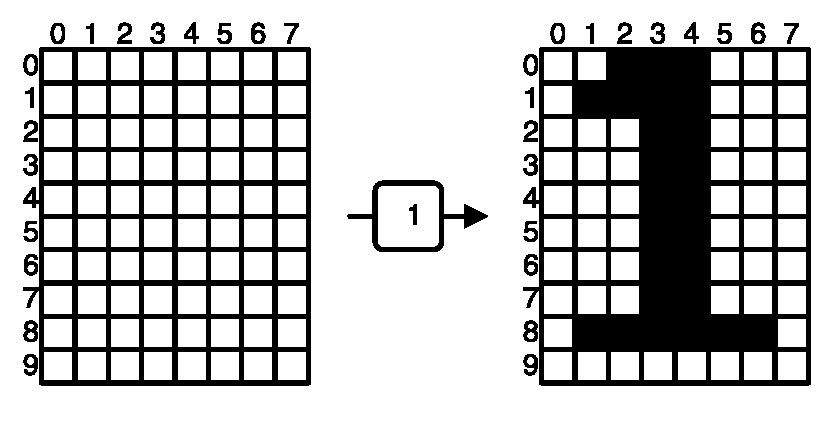
\includegraphics[scale=0.5]{./figures/matrix_font.pdf}
    \end{center}
    \caption{Esempio della mappatura di un carattere del font}
    \label{fig:matrix_font}
\end{figure}

È noto che non esiste una funzione come la \texttt{printf} su microcontrollori, e di conseguenza
neanche per stampare una stringa sullo schermo \texttt{ili9341} in quanto non vi è la conoscenza
ne di uno \textit{standard output} ne di un font. Quindi, è stato necessario trovare un font,
e di preciso abbiamo utilizzato un font che rappresentasse ogni glifo (simbolo o lettera) come
bitmap quindi in formato matriciale $8 \times 10$ pixel descrivendoli come 10 numeri a 8 bits.

In Figura \ref{fig:matrix_font} è possibile vedere come viene rappresentata graficamente
la matrice che rappresenta un carattere. Lato implementativo ogni riga viene tradotta in
un \texttt{uint8\_t} nel quale i bits settati a $1$ sono quelli che sono quelli colorati di nero,
per esempio la prima riga è tradotta in $0b00111000 \rightarrow 0d56$ il quale sarà il primo
componente del vettore che rappresenta il carattere $1$. Questa bitmap è passata alla
funzione
{\setmintedinline[c]{style=friendly}\inlinec{void WriteChar(struct ILI9341_t *ili, int X, int Y, int FW, int FH, unsigned char (*font)[FH])}}
sotto forma di vettore (\texttt{font}) lungo 10 di \texttt{unsigned char}.

Inoltre, abbiamo implementato delle funzioni ausiliarie. In particolare, la funzione
{\setmintedinline[c]{style=friendly}\inlinec{void WriteString(struct ILI9341_t *ili, int X, int Y, int FW, int FH, int N_GLYPHS, unsigned char (*font)[N_GLYPHS][FH], char *str)}}
che consente di stampare una stringa sullo schermo utilizzando la funzione
{\setmintedinline[c]{style=friendly}\inlinec{WriteChar}}. Questa funzione accetta in input
la posizione in cui stampare la stringa, la dimensione del font, il numero di glifi presenti
nel font e la stringa da stampare.

Abbiamo sfruttato queste implementazioni per stampare il menù di selezione, il quale
è composto da una lista di giochi presenti sulla scheda microSD suddivisi in varie pagine
e da una sezione per la selezione selezione per la velocità di esecuzione e la modalità
di esecuzione. La funzione accetta in input un array di stringhe, un array di modalità di
esecuzione e un array di velocità di esecuzione, e le restanti informazioni che servono
a {\setmintedinline[c]{style=friendly}\inlinec{WriteString}}.

\section{Assemblaggio}

\begin{figure}[h!t]
    \begin{center}
        % 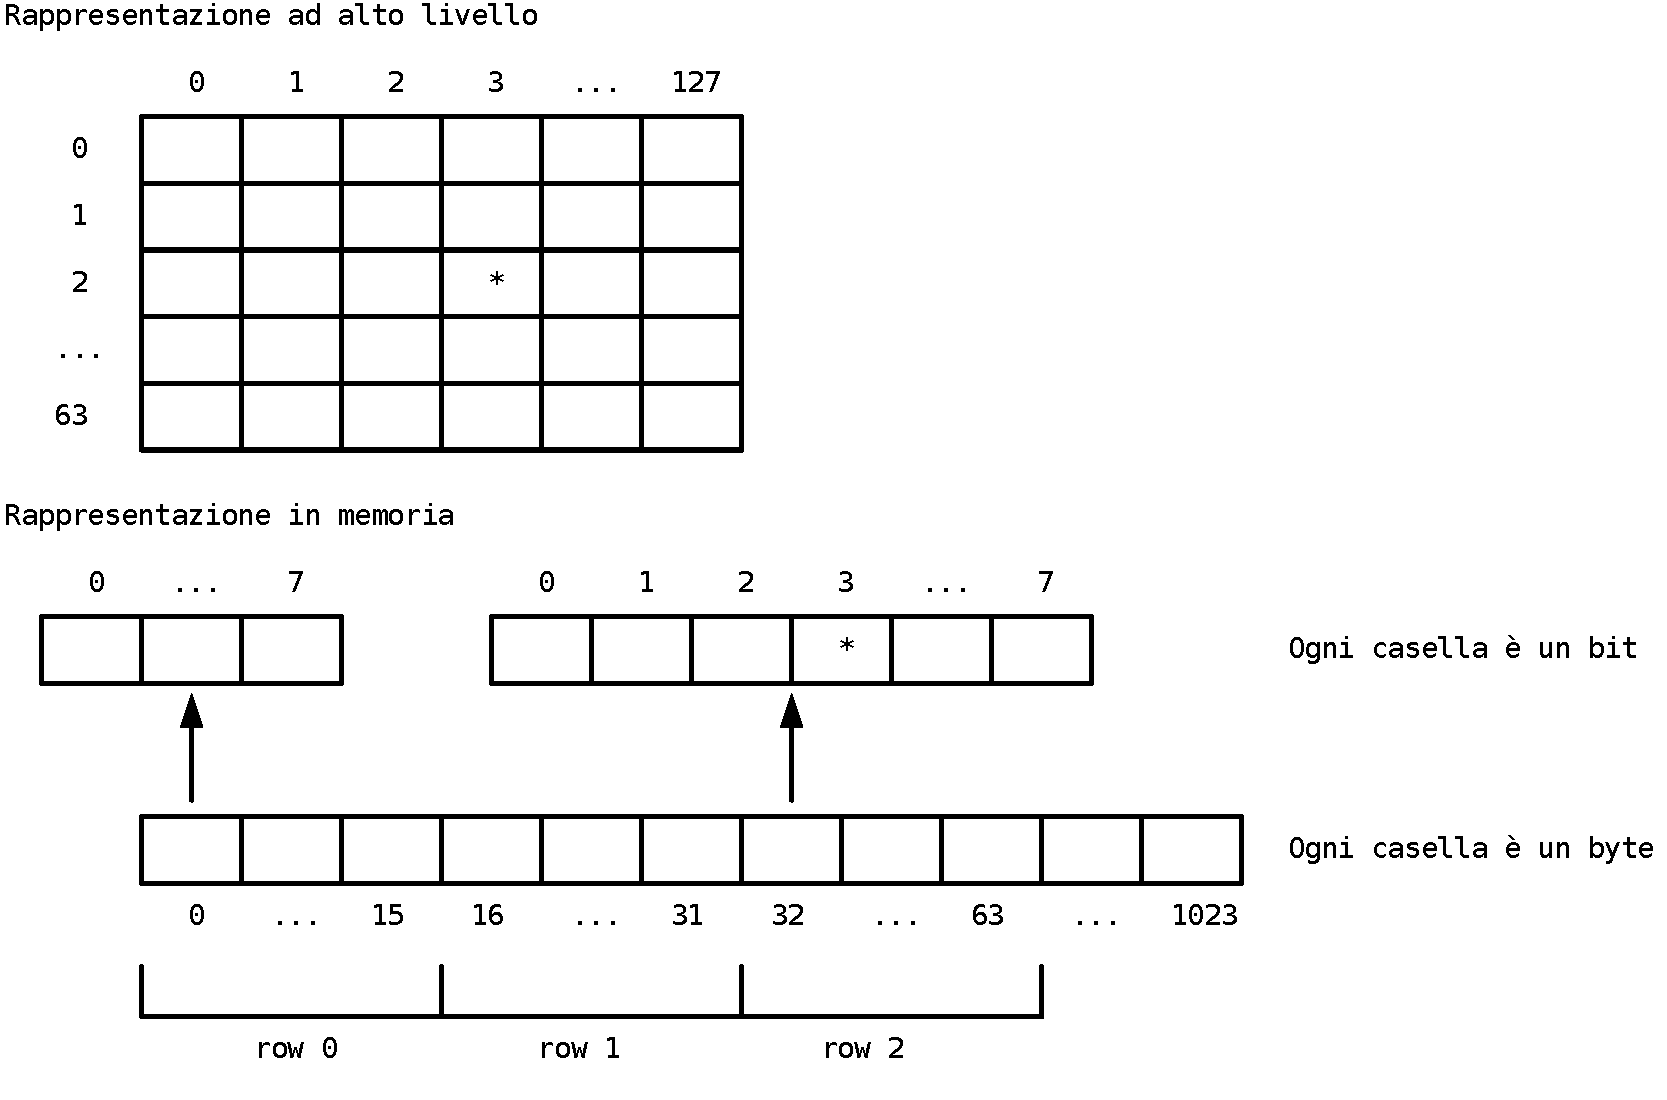
\includegraphics[scale=0.3]{figures/screenopt.pdf}
        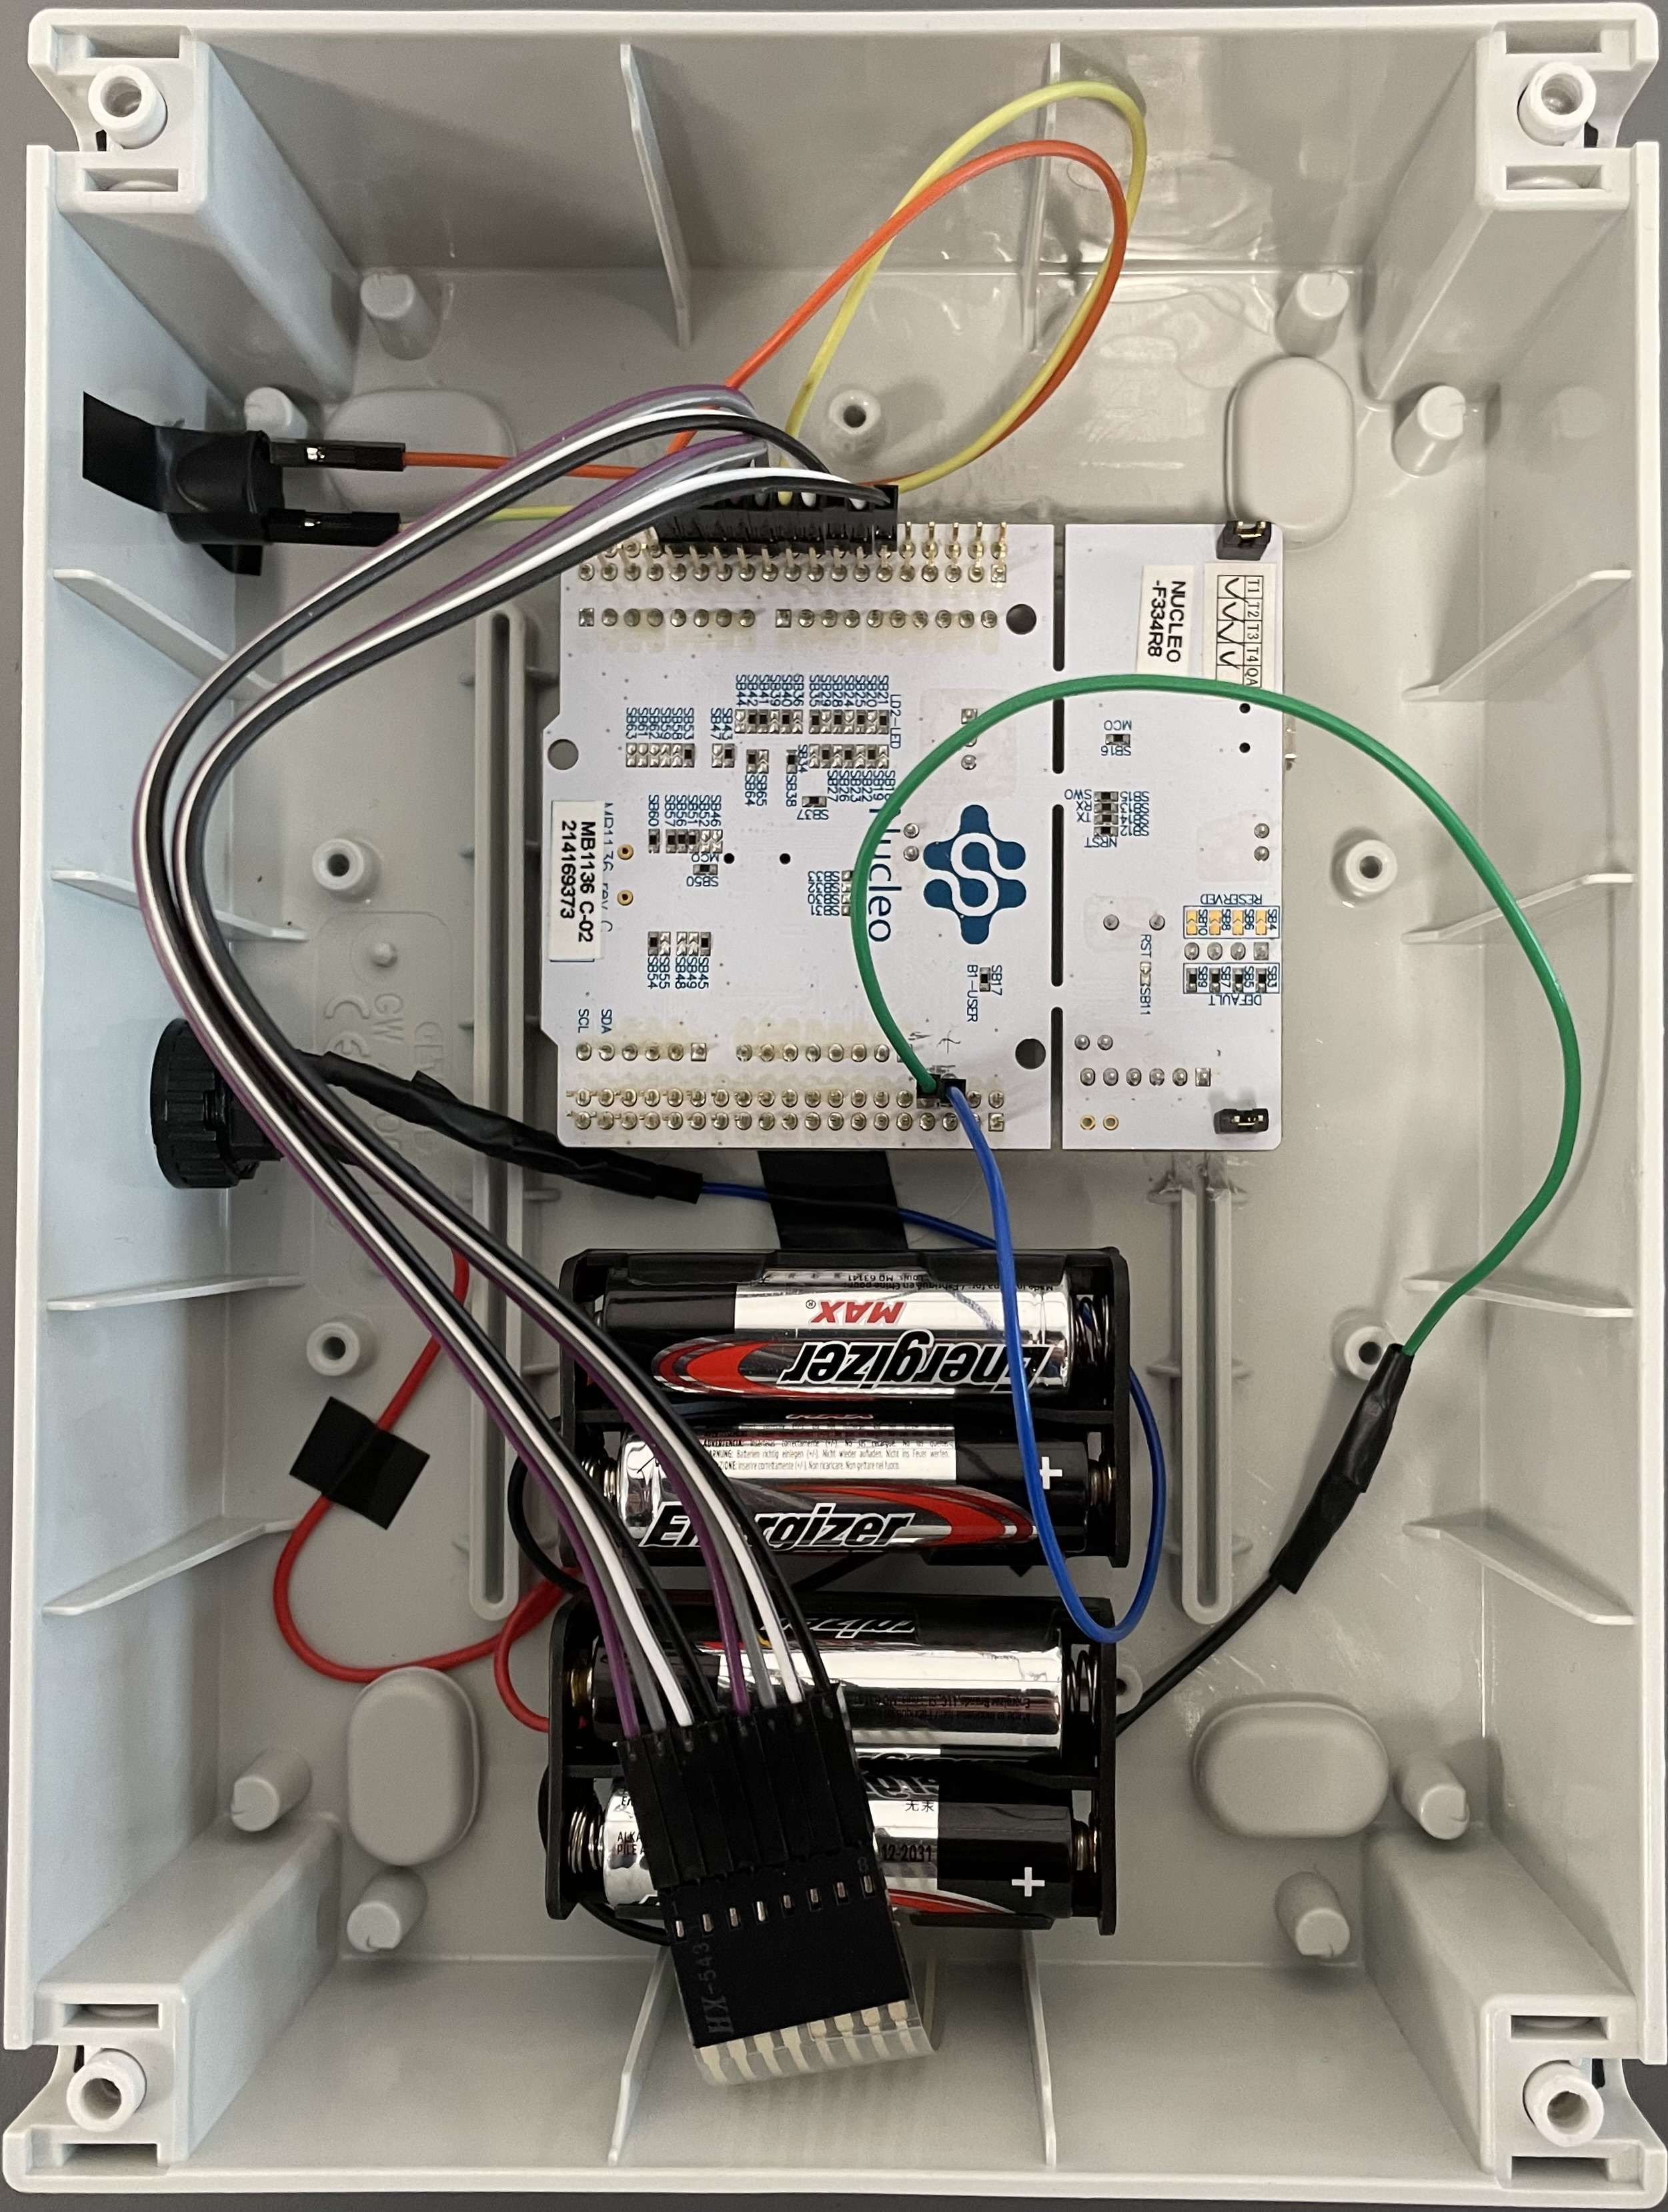
\includegraphics[scale=0.2]{./figures/end1.jpg}
        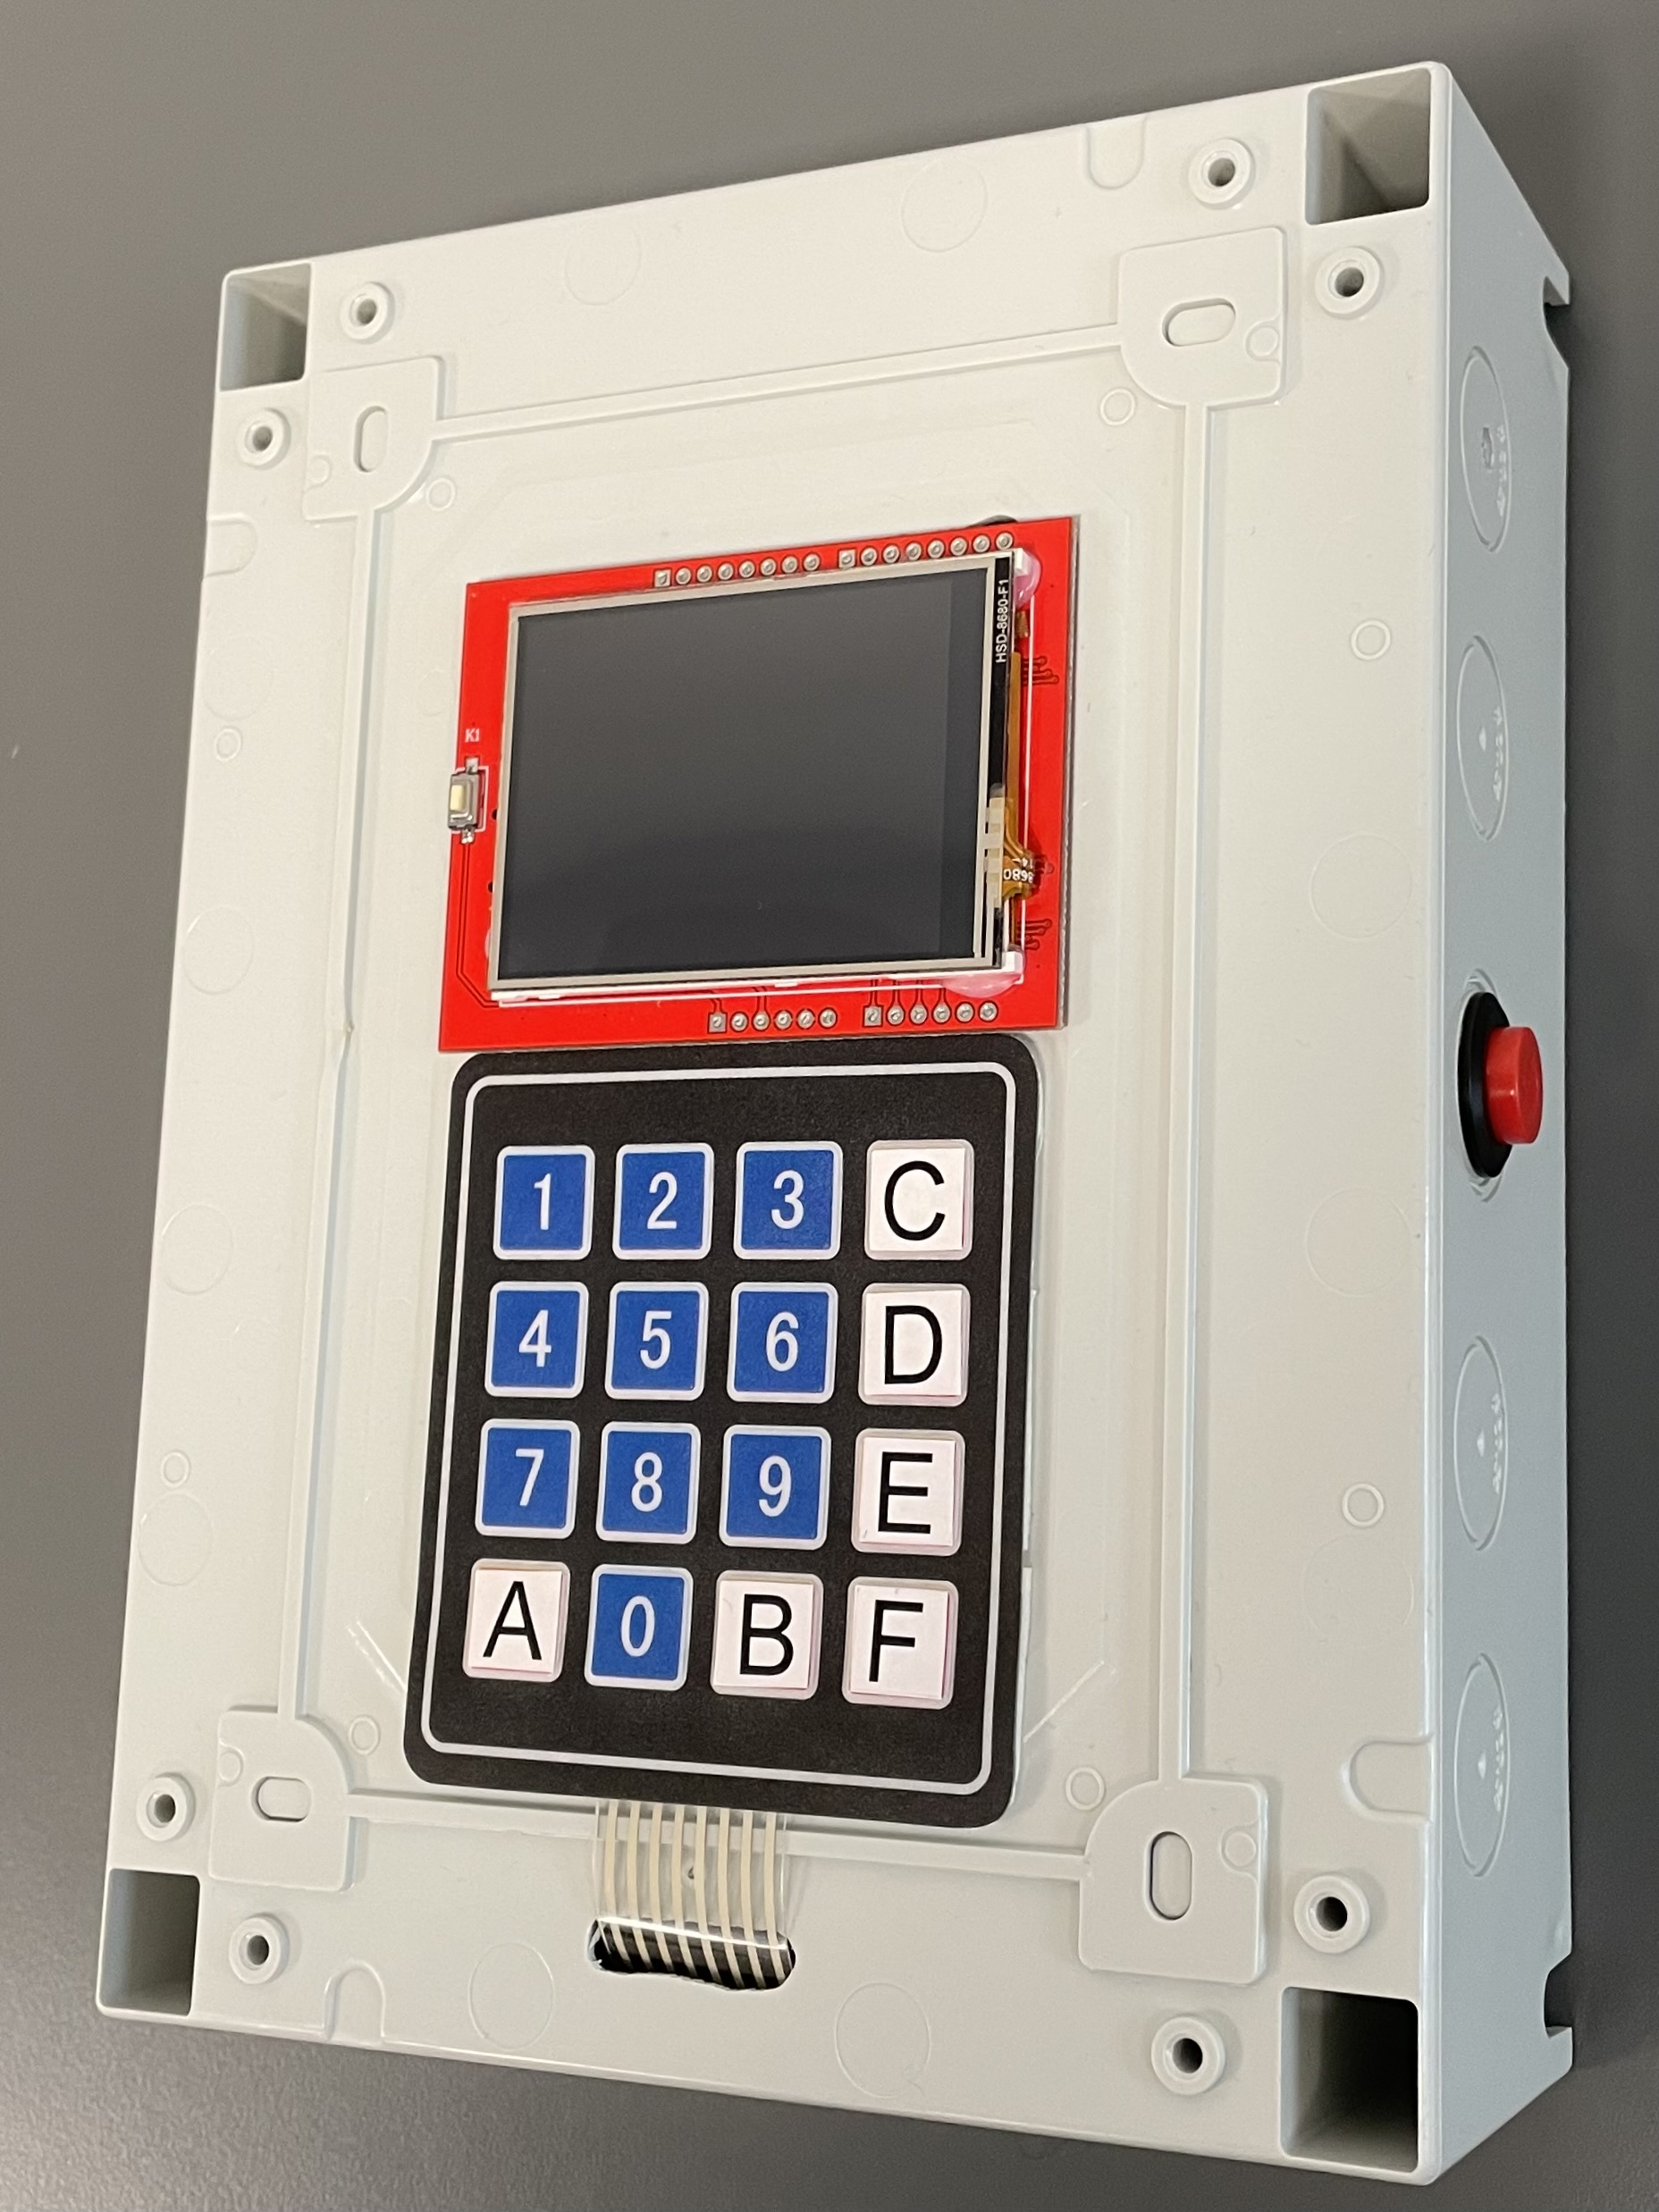
\includegraphics[scale=0.268]{./figures/end2.jpg}
        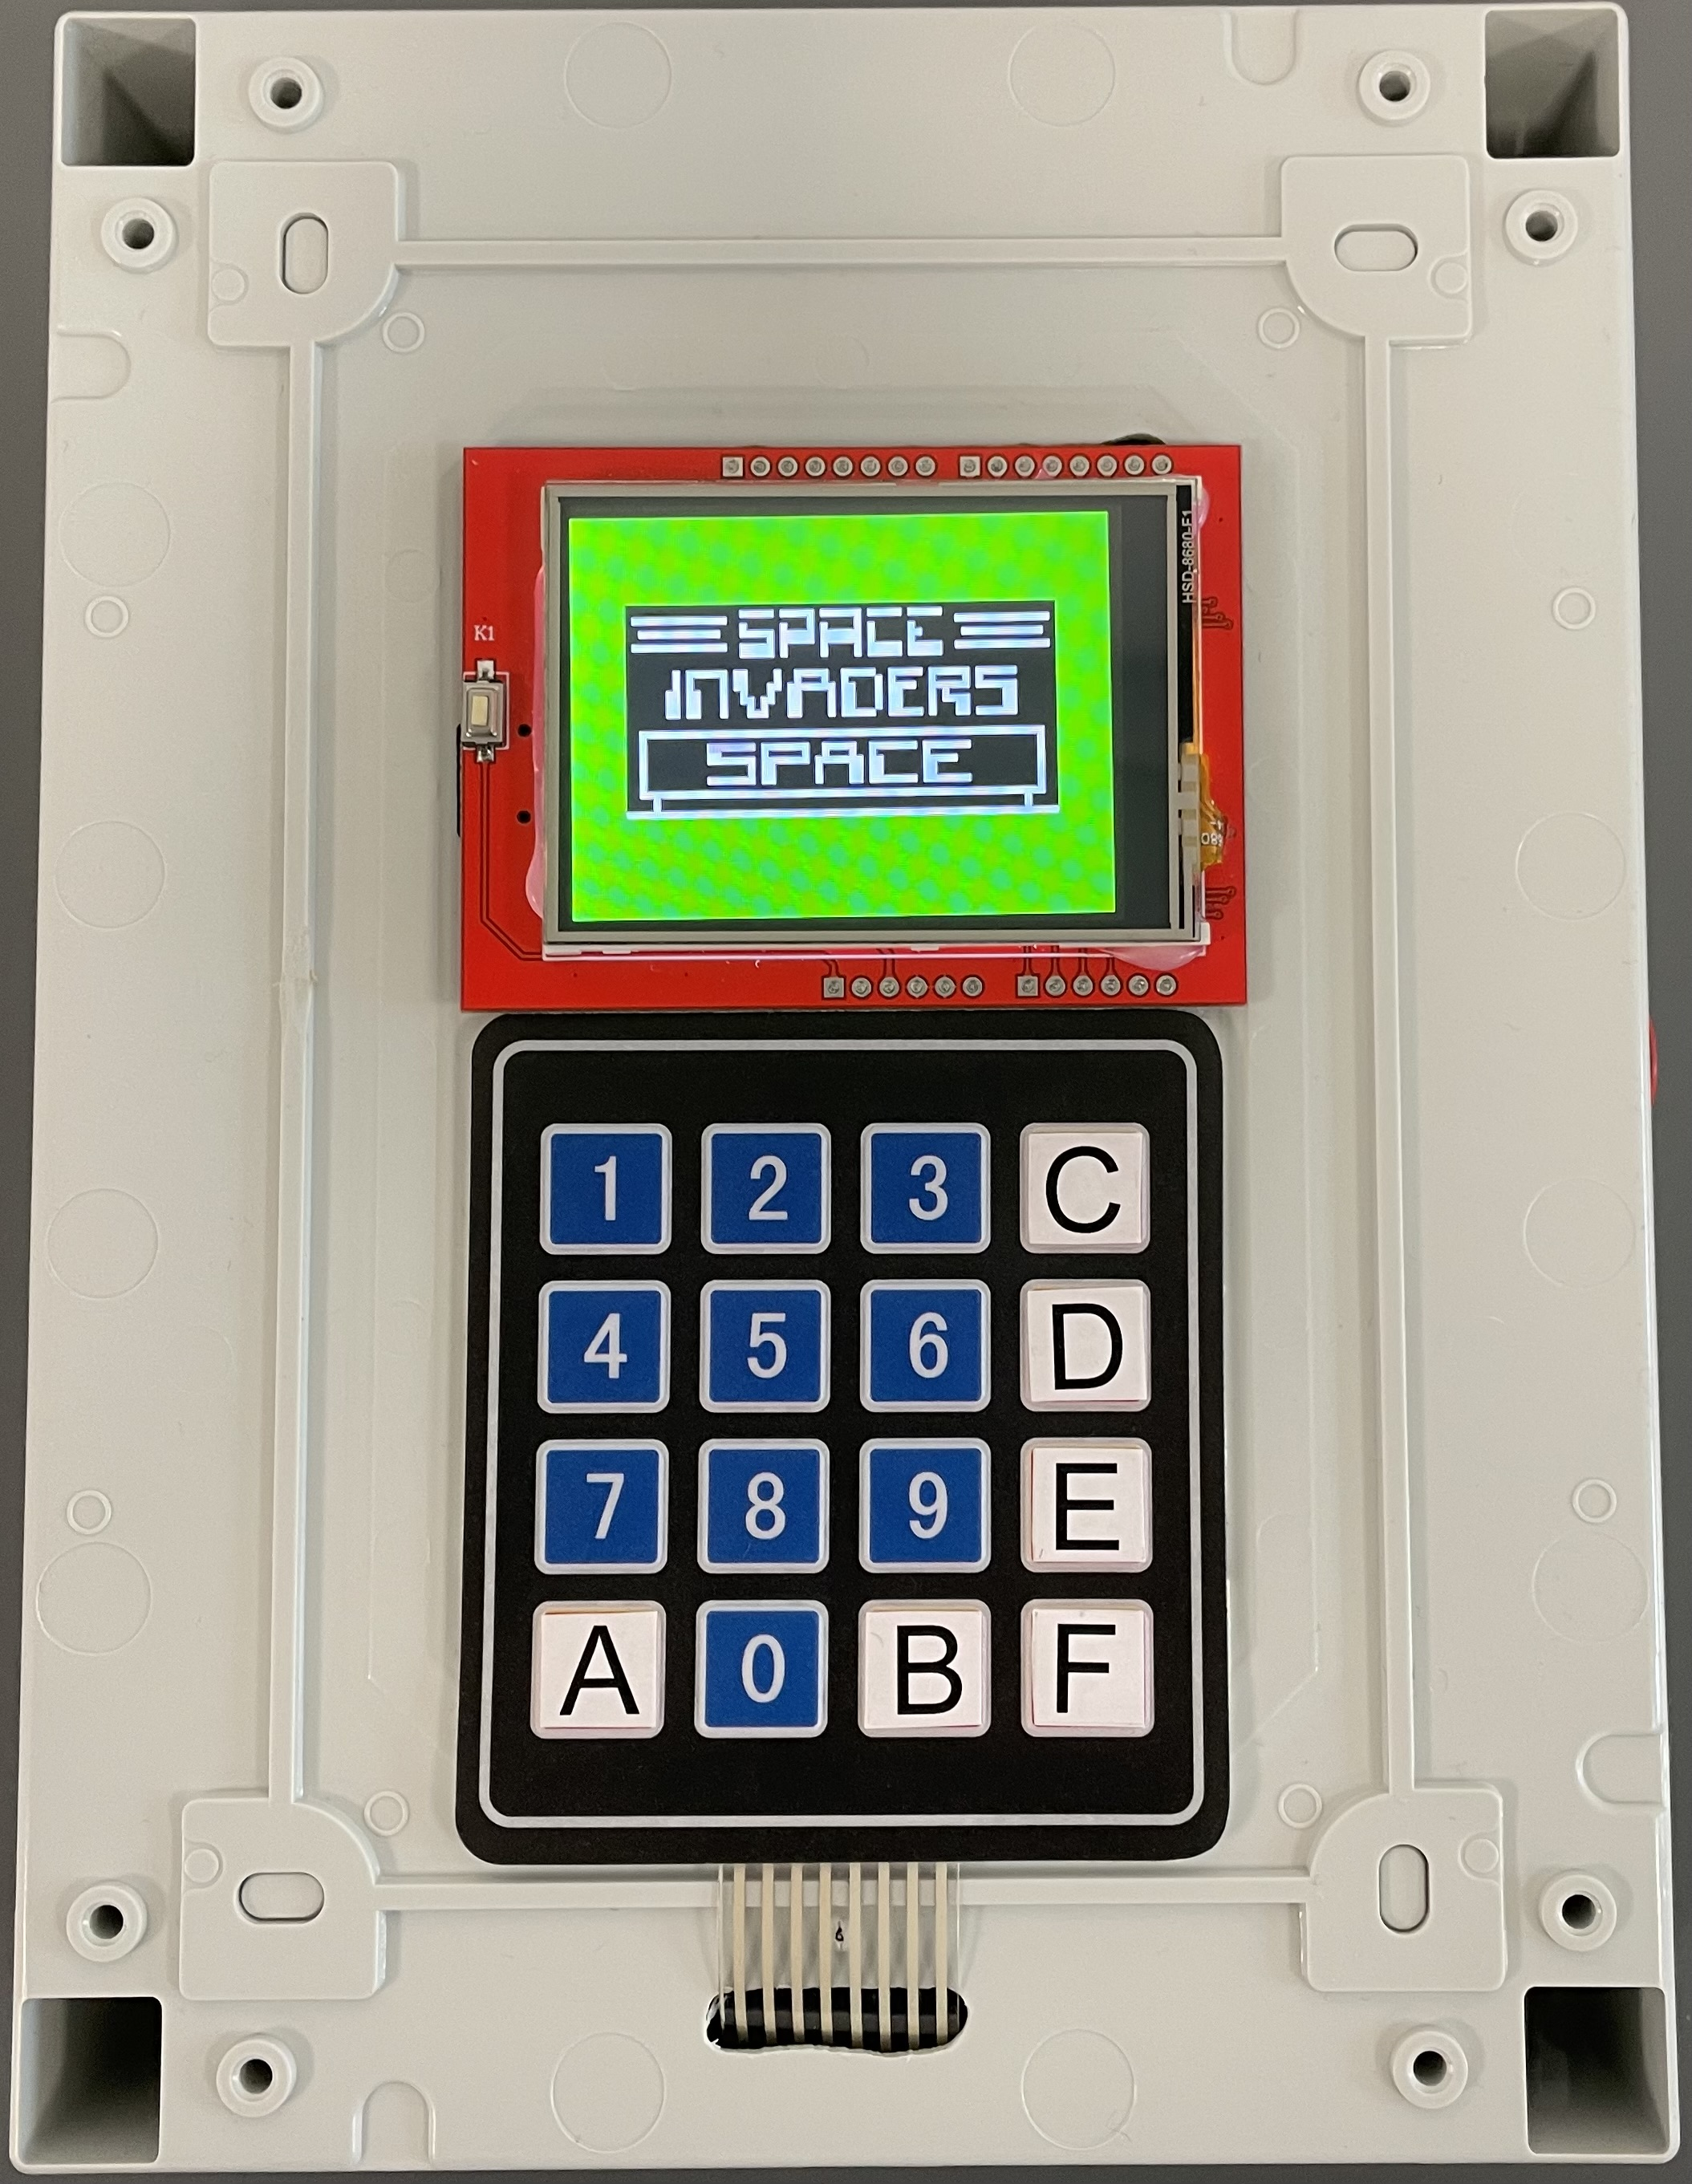
\includegraphics[scale=0.244]{./figures/end3.jpg}
    \end{center}
    \caption{Assemblaggio finale.}
    \label{fig:assemblaggio}
\end{figure}

Una volta terminato lo sviluppo del software abbiamo deciso di inserire i componenti hardware
all'interno di un guscio protettivo, in modo da nascondere il cablaggio e i vari pin scoperti,
lasciando accessibili solamente le parti con cui il giocatore interagisce direttamente.

Il guscio protettivo è stato realizzato con una base di supporto
polifunzionale\footnote{\url{https://www.gewiss.com/al/it/prodotti/product.1000002.1000090.GW42002}}
a cui sono state apportate le modifiche appropriate per essere in grado di "montare" correttamente
il display e il tastierino. Inoltre sono stati effettuati due fori sulla scocca per poter sentire
più facilmente il beeper e per poter accedere ad un interruttore per l'accensione e spegnimento
della scheda.

I collegamenti sono rimasti identici a quelli descritti nella sezione
\ref{subsubsec:collegamenti}, è stata però aggiunta una batteria esterna.

Infine, come ultimo tocco puramente estetico, abbiamo applicato degli adesivi al tastierino
per ricoprire i tasti che non corrispondevano a quelli originali del COSMAC VIP.

Consideriamo il risultato finale accettabile come prototipo iniziale, ma se si volesse
commercializzare un prodotto simile sarebbe imperativo utilizzare una PCB ad hoc più compatta,
un guscio su misura e un tastierino di qualità superiore.

\section{Analisi del consumo energetico} % FIXME

La scheda \texttt{STM32F334R8T6} può essere alimentata sia tramite un cavo USB che mediante
una batteria esterna; per rendere l'emulatore portatile abbiamo scelto quest'ultima
soluzione utilizzando 4 batterie AA da 1.5V ciascuna. Abbiamo collegato le batterie in
serie e connesso il polo positivo al pin VDD e il polo negativo al pin GND della scheda.

% FIXME
%
% Per ottenere una stima dell'autonomia dell'emulatore, abbiamo analizzato il suo consumo
% energetico utilizzando il software STM32CubeIDE. Il consumo energetico della scheda è di
% circa 30 mAh, mentre quello del display si aggira intorno ai 50 mAh per la retroilluminazione
% e 10 mAh per il display TFT. Quindi, complessivamente, l'emulatore consuma circa 90 mAh.

Per ottenere una stima dell'autonomia dell'emulatore, abbiamo analizzato il suo consumo
energetico utilizzando il software STM32CubeIDE. Il consumo energetico della scheda è di
circa 30 mAh, mentre quello del display retroilluminato si aggira intorno ai 90 mAh.
Quindi, complessivamente, l'emulatore consuma all'incirca 120 mAh.

Assumendo che le batterie abbiano una capacità di 2500 mAh, ci aspettiamo che
l'emulatore possa rimanere acceso per circa 20 ore.

\begin{equation*}
    \begin{aligned}
        \textmd{tempo} & = \frac{\textmd{capacità}}{\textmd{consumo}} & = \frac{2500}{120} & = 20
    \end{aligned}
\end{equation*}

\section{Considerazioni finali}

Siamo riusciti a realizzare un emulatore CHIP-8 e S-CHIP in grado di funzionare su un
microcontrollore STM32 raggiungendo così l'obiettivo che ci eravamo prefissati.

Alcuni videogiochi purtroppo non hanno un gameplay fluido a causa della potenza
limitata della scheda, nonostante questo Tetris, Blitz, Tic-tac-toe e altri giochi
analoghi hanno prestazioni più che accettabili.

Infine, per quanto riguarda possibili sviluppi futuri abbiamo ipotizzato che si potrebbe
ulteriormente ottimizzare il software modificando l'interprete in modo tale da interagire
direttamente con il display, perdendo però così la sua portabilità.

% TODO - sistemarlo e spostarlo
%
% Abbiamo ipotizzato una possibile ottimizzazione che permetta di aggiornare solo la sprite
% effettivamente modificata rispecchiando così il modo in cui vengono gestite le istruzioni
% che modificano lo stato dello "schermo" all'interno dell'interprete. Purtroppo però questo
% non è possibile perché, soprattutto quando l'emulatore è settato ad una frequenza alta,
% è possibile che più istruzioni di disegno vengano eseguite durante un ciclo di emulazione,
% per questo motivo siamo forzati a renderizzare lo "schermo" dell'interprete nella sua interezza.

\addcontentsline{toc}{section}{Riferimenti bibliografici}
\bibliographystyle{plain}
\bibliography{report}

\end{document}

